%!TEX root = ../thesis.tex
%*******************************************************************************
%****************************** Third Chapter **********************************
%*******************************************************************************
\chapter{Causal Abstractions}\label{chapter:causality}

% **************************** Define Graphics Path **************************
\ifpdf
    \graphicspath{{Chapter3/Figs/Raster/}{Chapter3/Figs/PDF/}{Chapter3/Figs/}}
\else
    \graphicspath{{Chapter3/Figs/Vector/}{Chapter3/Figs/}}
\fi

\emph{This chapter is largely based on the paper:}


\begin{quote}
\fullcite{rubenstein2017causal_fullcite}.
\end{quote}

%\citep{rubenstein2017causal}
%\cite{rubenstein2017causal}
%\citet{rubenstein2017causal}

\emph{Additional, the following paper on theme of causality was published during my PhD but is not included in this thesis:}

\begin{quote}
\fullcite{rubenstein2018deterministic}
\end{quote}

\emph{as well as the following workshop papers:}

\begin{quote}
\fullcite{rubenstein2017probabilistic}
\end{quote}

\begin{quote}
\fullcite{von2019optimal}
\end{quote}

\emph{Sections ... are an in-depth introduction to causality, motivating and explaining the setting considered by the paper.
Sections ... are mostly based on the paper. 
Section ... discusses how this work has influenced the research community and briefly discusses work that builds on it.}



\section{Introduction}

Much of machine learning concerns the statistical relationships between random variables. In this context, the word \emph{statistical} refers to the assumptions that a fixed but unknown probability distribution exists from which observed data are sampled \emph{independently and identically distributed (\iid)}, and that new data at `test time' will similarly be drawn \iid~from this distribution.
Classification is the canonical example of this, where given a set of \iid~samples from a joint distribution $\PP_{XY}$ over input $X$ and discrete target $Y$, the goal is to learn the conditional distribution $\PP_{Y|X}$ giving the probability distribution over targets for each possible input. Other problems such as density estimation can be phrased similarly.
%Given a set of \emph{i.i.d.} samples from a distribution $\PP_X$, the goal of \emph{density estimation} is to learn an approximation to $\PP_X$.

Despite the great empirical successes of machine learning in practical and applied settings in recent years, there remain problems of interest that cannot be cast directly into the framework described above. 
The framework is limited in that it presupposes the existence of a single joint distribution over all of the random variables of interest, with the operations of marginalisation and conditioning then providing the relationships connecting any subset of variables.
But there are many examples of problems for which a single joint distribution over all variables does not suffice. 
For many questions of scientific interest, this is because the problem either implicitly or explicitly concerns an \emph{intervention} or \emph{action} in the world that changes the joint distribution over the observable variables.

For example, we may be interested to understand the influence of diet on longevity, with the aim of improving public health by encouraging people to eat healthily. 
One might find the consumption of expensive imported fruits to be correlated with a longer life. This may well be due to the nutritiousness of such fruits; it could equally well be due to the fact that only wealthy people can afford such a diet, and that such wealth entails better access to medical treatment, sports facilities for exercise and so on. In the former case, intervening in the world by reducing tariffs on imported fruits to make them cheaper and thus encourage their consumption would have a positive effect on public health; in the latter, not.
Similarly, we may observe in the population that taking over-the-counter painkillers is associated with an elevated risk of heart disease. This might be because such painkillers have a negative effect on the cardiovascular system, in which case acting to reduce access to such painkillers might have a positive impact on health outcomes. But if instead the association is because people who have poor health, and thus heightened risk of heart disease, tend to take more painkillers, then such a policy might have little effect other than to increase overall suffering.

These questions are concerned with understanding causal, not statistical, relationships in the world. 
The aim of \emph{causality} is to study causal influence through the lens of a formal mathematical language, in much the same way that statistical machine learning uses the language of probability. 
\emph{Causal inference} or \emph{causal discovery}, a large part of the causality literature, concerns the identification of causal relationships using data.
As the examples above demonstrate, this can be highly non-trivial, with the well-known phrase ``correlation does not imply causation'' standing testament to the simultaneous difficulty and ubiquity of this problem.
Since correlation (or statistical dependence more generally) is a symmetric relation, an asymmetric causal relationship between two variables can never be inferred without other prior knowledge. 
Moreover, simply identifying that two quantities tend to co-occur does not itself imply a causal relation between the two, since both could be causally influenced by a third.

While causal inference is an important problem with a wide variety of applications ranging from astronomy to neuroscience and economics \citep{scholkopf2016modeling, ding200617, hicks1980causality}, the main contribution of this chapter is to extend and provide greater understanding of \emph{Structural Equation Models (SEMs)}, one of the popular mathematical frameworks for formalising causal relationships between random variables and interventions, along with the variety of probability distributions these entail. 
In particular, this work seeks to understand the implications of modelling causal structure at a different level of \emph{abstraction} compared to the `truth'. For instance, causal influence between variables of interest may be mediated by irrelevant variables that are ignored; interactions between low-level variables may instead be modelled at a macroscopic level, similar to the manner in which temperature and pressure arise as macroscopic properties of a large number of gaseous particles; and though time invariably plays a role in any causal influence in the real world, mathematical models of causal structure may often omit explicit reference to it.
This work additionally sheds new light on \emph{cyclic} SEMs, a previously poorly understood family of causal models, and has implications to existing causal inference algorithms by providing a framework for understanding the limitations of previous approaches.

REWRITE:
The next sections provide a comprehensive background sufficient to understand the novel contribution of this chapter.
In Section ??, we will introduce SEMs, followed in Section ?? by an overview of approaches to causal inference using SEMs. 
In Section ?? we will discuss the implicit assumptions in these approaches to causal inference, which will lead us to discussing causal abstractions in Sections ?? to ??.
Section ?? discusses the influence that this work has had on the research community in the $\sim 2$ years since its publication as well as recent work by others that directly builds on it.

%Best summarised by the well known phrase ``correlation does not imply causation'', while causal influence between two random variables typically implies statistical dependence, the reverse is not true.
%At its heart, causality and statistical machine learning differ in that the former concerns itself with interventions in the world. 





%\begin{itemize}
%\item There are interesting problems that don't fall into above framework that are nonetheless about learning from data.
%\item For instance scientific questions that are causal in nature, which scientists investigate by gathering and analysing data. These often are to do with decision making. For instance, given a patient with some condition, should we give them drug A or drug B? Here we are interested in the causal influence of the choice of drug on health outcome, not the statistical correlations. The reasons for this are best illustrated with an example.
%\item Suppose that drug A is a well established treatment for a condition, while drug B is new and experimental. It may be that only those patients that are very  
%\end{itemize}


\section{Structural Equation Models: A Language for Causality}

\emph{This section introduces Structural Equations Models (SEMs), a mathematical formalism used to model causal influence. Later in the chapter an extension to the classical SEM will be presented.
We will avoid going into measure-theoretic detail here, and point the reader to \cite{bongers2016structural} for a more rigorous measure theoretic introduction to SEMs.}
\\

\noindent An SEM over a tuple of random variables $X = (X_1, \ldots, X_N)$ consists of equations so that each $X_i$ is written as a function of a subset of the other $X_j$ and an \emph{exogenous noise variable} $E_i$. More formally:

\medskip

\begin{definition}[Structural Equation Model (SEM)]\label{def:causality-classical-sem}
Let $X = (X_1, \ldots, X_N)$ and $E = (E_1, \ldots E_N)$ with each $X_i$, $E_i$ taking value in $\R$. An SEM $\mathcal{M}_X$ over $X$ is a tuple $(\mathcal{S}_X, P_E)$ where
\begin{itemize}
	\item $\mathcal{S}_X$ is a set of structural equations of the form $X_i = f_i(X_{\pa(i)}, E_i)$ for $i=1,\ldots,N$, where 
%the functions $f_i$ are measurable], 
$\pa(i) \subset \{1,\ldots,N\}$ and $X_{\pa(i)}$ is the corresponding subset of the variables $X$.
	\item The variables $E = (E_1,\ldots,E_N)$ have distribution $P_E$ which factorises, i.e. the $E_i$ are independent.
	\item The \emph{causal graph} $\mathcal{G}$, the directed graph with nodes $X_i$ and edges $X_i \to X_j$ if and only if $i \in \pa(j)$, is acyclic.
\end{itemize}
\end{definition}

%\paragraph{Remark:}
The requirement that $\mathcal{G}$ be acyclic ensures that the SEM implies a well defined distribution $\mathbb{P}_X$ over the variables $X$. This is known as the \emph{observational distribution}.
%We will discuss this fact further next. Later, we will discuss the additional fact that, in combination with the requirement that the noise variables $E_i$ are independent, $\mathcal{G}$ being acyclic implies a correspondence between the conditional independence properties of the joint distribution $\mathbb{P}_X$ and $\mathcal{G}$, which is useful for learning $\mathcal{G}$ from data (i.e. causal inference). 

\medskip

\begin{lemma}[Well defined observational distribution]\label{lemma:acyclic-sem-well-defined-obs-dist}
An SEM implies a well-defined observational distribution $P_X$ over $X$.
\end{lemma}

\begin{proof}
For any particular value $e$ of the noise variables $E$, there is a unique vector $x_e$ so that $(x_e, e)$ solves the structural equations $\mathcal{S}_X$. To see this, observe that acyclicity of $\mathcal{G}$ means that the structural equations can be solved recursively, beginning with variables with no parents. It follows that each $x_i$ can be written as a function of $e_{\text{anc}(i)}$, where $\text{anc}(i)$ are the indices of the \emph{ancestors} of $X_i$ in $\mathcal{G}$, that is the $X_j$ for which there exists a path $X_j \to X_i$ using the edges in $\mathcal{G}$. 
Denote by $f(e) = x_e$ the function mapping from values of $e$ to the unique solution $x_e$.
Then $f$ in combination with $P_E$ induces the push-forward distribution $P_X := f_\# P_E$ over the $X$-variables, i.e.\:$P_X$ is the distribution of the random variable $f(E)$, a function of the random variables $E$.
\end{proof}

As discussed in the introduction, an important part of causal relationships is a notion of behaviour under \emph{interventions}. SEMs are equipped with a formal notion of such interventions which we call \emph{perfect interventions}. The idea is that intervening on a variable makes a change to the function determining its value in the observational setting.  Although there may be an effect on the distributions over variables downstream of the intervened variable, the functions determining those variables are unchanged. Such an intervention is realised simply by replacing the structural equation of the intervened variable. This notion is easily generalised to interventions on multiple variables by replacing all of the corresponding equations. 

\medskip

\begin{definition}[Perfect interventions and the do-operator]
	Let $\mathcal{M}_X$ be a SEM, $i \in \{1,\ldots,N \}$ and $x_i \in \mathbb{R}$. The perfect intervention setting $X_i$ to take value $x_i$ is denoted $\doop(X_i = x_i)$ and is implemented by replacing the $i$th equation with $X_i = x_i$. The resulting set of structural equations is denoted $\mathcal{S}_X^{\doop(X_i=x_i)}$ and the resulting SEM $\mathcal{M}_X^{\doop(X_i=x_i)} = (\mathcal{S}_X^{\doop(X_i=x_i)}, P_E)$.
	Perfect interventions over two or more variables are also valid, which are denoted for instance as $\doop(X_i = x_i, X_k = x_k)$.
\end{definition}

%\paragraph{Remark:} 
We note in passing that the notion of a perfect intervention may also be extended to \emph{imperfect} or \emph{stochastic interventions} in which the intervened variable is set equal to some random variable rather than a constant. Formally, this is no different from the case of perfect interventions other than needing to additionally introduce distributions over the new random variables. 
%We will not discuss such interventions further. [cite Eberhardt? See elem causality book for references].

%\paragraph{Remark:} 
An intervened SEM is still just a SEM, since it has structural equations and a distribution over exogenous variables. The only difference is that the functions corresponding to an intervened variable $X_i = f_i(X_{\pa(i)}, E_i)$ will have $\pa(i) = \emptyset$ and $f_i$ will be a constant function. Moreover, the causal graph $\mathcal{G}_{\doop(\cdot)}$ has the same nodes but a \emph{subset} of edges compared to $\mathcal{G}$, and thus inherits acyclicity. This implies the following lemma.

\medskip

\begin{lemma}[Well defined interventional distribution for any perfect intervention]\label{lemma:acyclic-sem-well-defined-int-dist}
	Any perfect intervention $\doop(\cdot)$ on a SEM (i.e. any subset of variables set to any particular values) implies a well-defined interventional distribution $\mathbb{P}^{\doop(\cdot)}_X$ over $X$.
\end{lemma}
\begin{proof}
	As discussed in the remark above, $\mathcal{M}_X^{\doop(\cdot)}$ is a valid SEM. Thus, Lemma \ref{lemma:acyclic-sem-well-defined-obs-dist} applies to $\mathcal{M}_X^{\doop(\cdot)}$.
\end{proof}
	
SEMs can thus be thought of as a way to model not just a single distribution over the variables of interest, but an entire family of related distributions, one for each possible perfect intervention.
This is illustrated in the following simple example.

\begin{example}\label{example:causality-simple-sem}
Consider the SEM $\mathcal{M}_X=\{\mathcal{S}_X, P_E\}$ where
%
\begin{align*}
\mathcal{S}_X &= \big\{  X_1 = E_1,\ X_2 = X_1 + E_2\big\} \\
P_E &= \mathcal{N}\left(\begin{pmatrix}
0 \\
0 
\end{pmatrix}, 
\begin{pmatrix}
1 & 0 \\
0 & 1
\end{pmatrix}\right)
\end{align*}
%
Then the observational distribution is given by 
%
\begin{align*}
P_X = \mathcal{N}\left(\begin{pmatrix}
0 \\
0 
\end{pmatrix}, 
\begin{pmatrix}
1 & 1 \\
1 & 2
\end{pmatrix}\right)
\end{align*}
%
while the interventional distributions corresponding to $\doop(X_1 = x_1)$ and $\doop(X_2 = x_2)$ are given by the degenerate Gaussians
%
\begin{align*}
P^{\doop(X_1 = x_1)}_X &= \mathcal{N}\left(\begin{pmatrix}
x_1 \\
x_1 
\end{pmatrix}, 
\begin{pmatrix}
0 & 0 \\
0 & 1
\end{pmatrix}\right) \\
P^{\doop(X_2 = x_2)}_X &= \mathcal{N}\left(\begin{pmatrix}
0 \\
x_2 
\end{pmatrix}, 
\begin{pmatrix}
1 & 0 \\
0 & 0
\end{pmatrix}\right).
\end{align*}
\end{example}

\subsection{Connections to Bayesian networks}

SEMs are closely related to Bayesian networks, a class of graphical models.

\medskip

\begin{definition}
A Bayesian network over variables $X = (X_1,\ldots, X_N)$ with directed acyclic graph $\mathcal{G}$ specifies a joint distribution over $X$ as a product of conditional distributions
\begin{align*}
	p(X_1,\ldots,X_N) = \prod_{i=1}^N p(X_i | X_{\pa(i)})
\end{align*}
where the nodes of $\mathcal{G}$ correspond to the variables $X$ and there is an edge $X_j \to X_i$ in $\mathcal{G}$ if and only if $j \in \pa(i)$.
\end{definition}

Since any product distribution can always be decomposed as $p(X_1,\ldots,X_N) = \prod_{i=1}^N p(X_i | X_{j<i})$, it is the \emph{absence} of edges in $\mathcal{G}$ that imposes structure on the probability distribution.

Bayesian networks can be endowed with a similar notion of perfect intervention as SEMs. To model the effect of the perfect intervention $\doop(X_i = x_i)$, in the resulting joint distribution the factor $p(X_i | X_{\pa(i)})$ is replaced with a Dirac delta distribution $\delta_{X_i = x_i}$. 
Bayesian networks equipped with such a notion are often referred to as \emph{causal} Bayesian networks. 
In the following, we will simply refer to them as Bayesian networks.


\subsubsection{Correspondence between SEMs and Bayesian networks} 
SEMs and Bayesian networks exist in correspondence with one another. 
For any SEM, there exists a Bayesian network over the same variables that induces the same observational and interventional distributions, and vice versa.
We briefly explain this correspondence.

Any SEM induces a Bayesian network with the same graph $\mathcal{G}$.
To see this, observe that for any fixed value of $X_{\pa(i)}$, the equation $X_i = f(X_{\pa(i)} , E_i)$ in combination with the distribution over $E_i$ induces a distribution over $X_i$ which corresponds to $p(X_i | X_{\pa(i)})$. The observational distributions of the SEM and Bayesian network are then equal. Further, since the equation $X_i=x_i$ associated with the intervention $\doop(X_i = x_i)$ corresponds to the distribution $\delta_{X_i = x_i}$, and similar for interventions or arbitrary subsets of variables, the interventional distributions also agree.

Showing that any Bayesian network induces a SEM is somewhat more technical, and is outlined here based on the proof of Proposition 7.1 from \cite{peters2017elements}. 
For each $X_i$ with parents $X_{\pa(i)}$, define the function
%
\begin{align*}
F_{X_i|X_{\pa(i)}}:\mathbb{R} \to [0,1]
\end{align*}
%
to be the cumulative distribution function of $p(X_i|X_{\pa(i)})$ as given by the Bayesian network.
Define the exogenous variables of the SEM $E_1, \ldots, E_N$ to be uniformly distributed on the interval $[0,1]$, and let the structural equations be defined by
%
\begin{align*}
X = f_i(X_{\pa(i)}, E_i) := F^{-1}_{X_i|X_{\pa(i)}}(E_i).
\end{align*}
%
To see that this SEM induces the same observational distribution over the variables $X$ as the Bayesian network, it suffices to note that the conditional distributions $X_i|X_{\pa(i)}$ are the same for both the Bayesian network and the SEM, by definition of the cumulative distribution function.
Similarly, replacing any equation with $X_i=x_i$ corresponds to the cumulative distribution function associated to $\delta_{X_i=x_i}$ and so any interventional distributions also agree.


%is somewhat more complicated. In the case that all variables are discrete, this can be shown relatively straightforwardly \cite{druzdzel1993causality}. The intuition is that for any fixed value for $x_{\pa(i)}$,  the distribution $p(X_i | X_{\pa(i)}=x_{\pa(i)})$ can be written as a transformation $g_{x_{\pa(i)}}(E_i)$ of a uniformly distributed random variable $E_i$. We can then define the function $f_i$ of the constructed SEM as $f_i(x_{\pa(i)}, e_i) = g_{x_{\pa(i)}}(e_i)$, which is straightforwardly measurable as all spaces are discrete. [**Check this**]

%In the general case, however, one quickly runs into very technical measure-theoretical arguments due to the requirement that the functions $f_i$ be measurable. [Basically, the issue is that you need to ensure that $E_i$ can be transformed into $p(X_i | X_{\pa(i)}=x_{\pa(i)})$ for all choices of $x_{\pa(i)}$. You get a different transformation$g_{x_{\pa(i)}}$ for each value of $x_{\pa(i)}$. Then you need to show that defining $f_i(x_{\pa(i)}, e_i) = g_{x_{\pa(i)}}(e_i)$ results in $f_i$ being measurable. If $f_i$ is continuous in each of its arguments then paper cited in second answer of \url{https://math.stackexchange.com/questions/215215/showing-a-function-of-two-variables-is-measurable} says that it is measurable. But in the general case I'm not sure what to do. 

%I think it suffices to say that in most typical use cases, the conditional probability distributions will be specified in some way that makes them amenable to directly rewriting as an SEM. For example, if conditional distribution is Gaussian with mean and covariance dependent on parents, the reparameterisation trick is precisely writing this as a SEM.]
%\\


\subsubsection{Differences between SEMs and Bayesian networks}

%There are some differences between SEMs and Bayesian networks, though it is easy to overstate these.
%It is easy to overstate the differences between SEMs and Bayesian networks. As the remark above discusses, they are fundamentally the same, with their main differences being mostly philosophical.
%
%SEMs are usually explicitly used with the modelling of causal structure in mind, while Bayesian networks are often not. For instance, variables in a Bayesian network may represent uncertain parameters or latent variables that have no direct physical meaning.
%
In an SEM the noise variables $E$ are explicitly modelled, while in a Bayesian network they are not.\footnote{An exception to this is the \emph{reparameterisation trick} as a way to train Bayesian networks via stochastic gradient methods \citep{kingma2013auto,rezende2014stochastic}, though as the name suggests this is generally viewed as a computational `trick' rather than a general strategy of mathematical modelling.}
As discussed in \cite{pearl2009causality}, this corresponds to a quasi-deterministic view of the world in which any observed randomness is a consequence of a lack of knowledge. In contrast, modelling with Bayesian networks corresponds to a view that the world is inherently stochastic.
%This difference is largely academic and we will not concern ourselves with it further.

As a consequence of the noise variables being explicitly modelled, SEMs are equipped with \emph{counterfactual reasoning}. 
That is, once the variables have been observed, the noise values for the variables can generally be inferred. 
This means that one can answer questions such as ``what would have happened had the intervention $\doop(X_i=x_i)$ been performed?''
%\paragraph{Example:} todo.
Whether or not this is useful in practice is debatable, since different SEMs may imply the same set of observational and interventional distributions, but nonetheless be counterfactually non-equivalent. That is, they may produce different answers to the same counterfactual question, despite implying the same observational and interventional distributions. This means that such models cannot be distinguished based on data, be it in the observational or interventional setting. Therefore one cannot hope to be able to answer counterfactual questions based 
on data without prior knowledge to distinguish between counterfactually non-equivalent models.
%We will not discuss counterfactual reasoning further.


There are two main consequential differences between SEMs and Bayesian networks.
First, it can be easier to express assumptions on the mechanisms of causal influence within the SEM framework, for instance by assuming that the distribution $P_E$ and the functions $f_i$ belong to some restricted sets.
Second, it is also conceptually simple to extend the SEM framework to express cyclic dependencies, which we discuss in the next section.
%For this reasons, study of the SCM framework is preferred in this chapter.

%Next, we discuss the relaxation of the acyclicity contraint in the definition

Mention latent confounders and that independent noise variables corresponds to no latent confounders?

\subsection{Cyclic Structural Equation Models}

Most causal systems in the real world involve some degree of feedback. 
Examples can be found in a wide variety of settings: molecular biology (e.g. gene-gene or gene-protein interactions in a cell), ecology (e.g. population dynamics), climate science (e.g. methane release from thawing permafrost) and public policy and economics (e.g. poverty traps).
Studying the mathematical modelling of these cases is interesting in part because their treatment requires consideration of issues that are not present in the acyclic, feedback-free case.

Recall that Lemmas \ref{lemma:acyclic-sem-well-defined-obs-dist} and \ref{lemma:acyclic-sem-well-defined-int-dist} relied on acyclicity of the causal graph $\mathcal{G}$ to prove that an SEM induces well-defined observational and interventional distributions over the variables $X$. 
When generalising to \emph{cyclic SEMs} by relaxing this acyclicity constraint, one must be careful to understand under which conditions the observational and interventional distributions are well-defined.
The implied observational distribution is well-defined if and only if there is a unique solution $X(E)$ to the structural equations for $P_E$-almost all values of $E$. Similarly, an interventional distribution is well-defined if and only if the intervened structural equations have unique solution $P_E$-almost surely.
The following example shows a simple case of an SEM with well-defined observational distribution for which some interventional distributions are well-defined but others are ill-defined.

\begin{example}\label{example:causality-cyclic-invalid}
Consider the cyclic SEM $\mathcal{M}_X=\{\mathcal{S}_X, P_E\}$ where
%
\begin{align*}
\mathcal{S}_X = \big\{  X_1 &= X_2 + X_3 + E_1, \\
					    X_2 &= X_1 + X_3 + E_2, \\
					    X_3 &= X_1 + X_2 + E_3\big\} \\
\end{align*}
%
and $P_E$ is any distribution.
In the observational setting, the values 
\[(X_1, X_2, X_3) = \left(\frac{E_2 + E_3}{2}, \frac{E_1 + E_3}{2}, \frac{E_1 + E_2}{2}\right)\]
uniquely solve the structural equations, and hence the observational distribution $P_X$ is well-defined. 

Under the intervention $\doop(X_1 = x_1)$, the equations have either infinitely many solution, in the case that $E_Y + E_Z = -2 x_1$, or zero solutions, if $E_Y + E_Z \not= -2 x_1$. 
Hence the interventional distribution $P_X^{\doop(X_1 = x_1)}$ is ill-defined, and similarly for other interventions on a single variable.

Under the intervention $\doop(X_1=x_1, X_2=x_2)$, the equations have unique solution 
\[(X_1, X_2, X_3) = \left(x_1, x_2, x_1 + x_2 + E_3 \right).\]
Thus the interventional distribution $P_X^{\doop(X_1 = x_1, X_2=x_2)}$ is well defined, similarly for any intervention on two variables.
\end{example}

%\todo{\paragraph{Example:} $X$, $Y$, $Z$ with $X = Y+Z+ E_X$ and so on. Then observational distribution is well defined with e.g. $X= -(E_Y + E_Z) / 2$. But interventional distributions on single variables are in general not well defined. Interventions on pairs of variables are well defined.}

The literature on cyclic SEMs has not settled on a set of criteria for which cyclic SEMs should be considered `valid'. 
All agree on the fact that observational distributions must be well-defined, but there is significant disagreement on interventional distributions.
Notable works include \cite{hyttinen2010causal}, which requires well-defined distributions after any intervention, and \cite{mooij2011causal}, which state that for any cyclic SEM, any intervention leading to a well-defined interventional distribution may be given a causal interpretation. Other works in this area such as \cite{lacerda2012discovering} avoid discussion of this issue.

It will be argued in Sections \ref{sec:causality-what-are-causal-vars} and \ref{sec:causality-transformations-between-sems} that it should be considered an integral part of the modelling process to choose a set of interventions being modelled. As such, it should be guaranteed that interventional distributions be well-defined for those that are part of the modelled intervention set; the behaviour outside of this set being considered outside of the universe and thus irrelevant.

\paragraph{Interpretations of cyclic SEMs}
Note to self: mention this later on after presenting transformations.
In the acyclic case, one can think of an SEM as defining a generative process in which variables are realised as a function of their parents. Interventions then break the generative process for a single variable, leaving other processes unchanged.
This interpretation breaks down for cyclic models. Existing works have interpreted them as dynamical systems that equilibrate quickly. 

%\iffalse
\section{Methods of Causal Inference}
\todo{The contents of this section aren't really relevant to the rest of the chapter. It seems weird to have a chapter on causality without mentioning causal inference though. I'm inclined to just remove it but leaving it visible for the meantime. I will not polish it further until I decide whether or not to keep it.}

Although the main contribution of this chapter is to improve theoretical understanding and extend the mathematical framework of SEMs, we discuss here the challenge of performing causal inference from observational data. %and outline some prominent methods for doing so, since this is ultimately of most interest to practitioners.
Generally speaking, the goal of a causal inference algorithm is to learn the causal graph $\mathcal{G}$. 
In the case of no latent confounders, once $\mathcal{G}$ has been identified, learning the functional relationships between parents and children reduces to solving independent regression problems. As such, we will only discuss methods for identifying $\mathcal{G}$, though some of these may estimate the functional relationships as an intermediate step.
These methods focus on the acyclic case unless otherwise stated.

More formally, the problem can be stated thus: Given \iid~draws from a distribution $\mathbb{P}_X$ induced by an SEM with causal graph $\mathcal{G}$, estimate $\mathcal{G}$.
Broadly speaking, there are two main categories of approaches: those which exploit a correspondence between statistical properties of $\mathbb{P}_X$ and properties of $\mathcal{G}$; and those that make additional assumptions on the noise variable distribution $\mathbb{P}_E$ and functions $f_i$.

\subsection{Conditional independence}

REWRITE:
At a high level, the idea is to relate statistical properties of the joint distribution $\mathbb{P}_X$ to properties of the causal graph $\mathcal{G}$.
The statistical properties in question are \emph{conditional independences}.
Graphs exhibiting the same set of conditional independences form an equivalence relation, the classes of which are known as \emph{Markov equivalence classes}.
From the conditional independences present in $\mathbb{P}_X$, it is thus possible to identify $\mathcal{G}$ up to its Markov equivalence class.
We begin by defining the notion of \emph{d-separation}, a purely graph theoretic concept. 
\\

\begin{definition}[d-separation]\label{def:d-sep}\citep{pearl2009causality}
Let $\mathcal{G}$ be a DAG with vertex set $V$ and define a \emph{path} to be a sequence of consecutive edges of either directionality. 
Let $Z \subset V$ and $u, w \in V \setminus Z$. 

$Z$ \emph{d-separates} $u$ and $w$ if and only if, for any path $p$
connecting $u$ and $w$, one of the following conditions holds:

\begin{itemize}
\item $p$ contains a chain $i \rightarrow m \rightarrow j$ or a fork $i \leftarrow m \rightarrow j$ such that $m \in Z$
\item $p$ contains a collider $i \rightarrow m \leftarrow j$ such that $m$ and all of its descendants
are not elements of $Z$.
\end{itemize}

Given disjoint subsets of variables $U$, $W$ and $Z$, we say that $Z$ \emph{d-separates} $U$ and $W$ if $Z$ d-separates $u$ and $w$ for all $u \in U$ and $w \in W$.
\end{definition}

The `d' stands for `directed', since this is a notion that holds only for directed acyclic graphs.
Intuitively, $Z$ d-separates two nodes $x$ and $y$ if conditioning on $Z$ blocks any flow of information between $x$ and $y$. That is, having already observed $Z$, learning the value of $x$ provides no extra information about the value of $y$ (and vice versa).

The following definition and theorem show how this graph theoretic notion is related to probability distributions.
\\

\begin{definition}[Markov]\cite{cite something?}
Suppose that $\mathcal{G}$ is a DAG with nodes corresponding to the tuple of variables $X$. 
A distribution $\mathbb{P}_X$ on $X$ is \emph{Markov} with respect to $\mathcal{G}$ if, for all
disjoint subsets $A$, $B$ and $C$ of $X$, 
\begin{center}
$A$ and $B$ are d-separated by $C$ $\implies$ $A \perp B | C$.
\end{center}
\end{definition}
\medskip

\paragraph{Remark:} if $\mathcal{G}'$ and $\mathcal{G}$ are two DAGs over the same vertices such that the edges present in $\mathcal{G}$ are a subset of those in $\mathcal{G}'$, then the set of d-separations entailed by $\mathcal{G}'$ is a subset of those entailed by $\mathcal{G}$. To see this, note that given any nodes $Z$, $u$ and $v$ in the definition, adding extra edges can only increase the number of paths $p$ that have to satisfy one of the conditions. 
This means that if $\mathbb{P}_X$ is Markov with respect to $\mathcal{G}$, it is also Markov with respect to $\mathcal{G}'$.
\medskip


\begin{theorem}\cite{lauritzen}
Suppose that $\mathbb{P}_X$ admits density $p(x)$ with respect to the Lebesgue measure, and that $\mathcal{G}$ is a DAG with nodes corresponding to the variables $X$ in which $X_i$ has parents $X_{\pa(i)}$. 
Then the following two conditions are equivalent:
\begin{enumerate}
\item $p(x)$ factorises as $p(x) = \prod_i p(x_i |x_{\pa(i)})$;
\item $\mathbb{P}_X$ is Markov with respect to $\mathcal{G}$.
\end{enumerate}
\end{theorem}
\medskip

Suppose that the distribution $\mathbb{P}_X$ is induced by an SEM with unknown graph $\mathcal{G}$.
The conditional independences exhibited by $\mathbb{P}_X$ constrain the set of possible graphs to which $\mathcal{G}$ must belong, since the d-separations that it entails must be consistent with the conditional independences.
However, the set of graphs with respect to which $\mathbb{P}_X$ is Markov is `too large', since $\mathbb{P}_X$ is Markov with respect to any DAG $\mathcal{G}'$ whose edges contain those of $\mathcal{G}$.
The following definition is a kind of minimality condition.\footnote{Faithfulness is additionally required to rule out certain pathological cases, for instance in which the influence of two variables on a third exactly cancel out. In the case of linear SEMs, such cases are rare \cite{lauritzen, see elem causality book ex. 6.34}.}
\\

\begin{definition}[Faithfulness]\cite{cite something?}
$\mathbb{P}_X$ is faithful with respect to $\mathcal{G}$ if, for all disjoint subsets
$A$, $B$ and $C$, 
\begin{center}
$A \perp B | C$ $\implies$ $A$ and $B$ are d-separated by $C$.
\end{center}
\end{definition}
\medskip

If $\mathbb{P}_X$ is both Markov and faithful with respect to a DAG $\mathcal{G}$, then there is an exact correspondence between the conditional independences of $\mathbb{P}_X$ and the Markov equivalence class of $\mathcal{G}$. 
This fact can be exploited for causal inference: give $\mathbb{P}_X$, identify the set of conditional independences and from this identify $\mathcal{G}$ up to its Markov equivalence class.
The most well-known algorithm that does this is the IC (inductive causality) algorithm.

The algorithm works by first constructing a `skeleton' of undirected edges, followed by orienting these edges.
For each pair of variables $u$ and $v$, one first searches for a set of other variables $Z_{uv}$ such that $u \perp v| Z_{uv}$. 
An undirected edge is drawn between $u$ and $v$ if no such $Z_{uv}$ can be found, since pair of nodes are adjacent if and only if there is a set that d-separates them \cite{elem causality, lemma 7.8}. 
The undirected arrows are then oriented as much as possible by identifying colliders ($u \rightarrow z \leftarrow v$).
This is done by exploiting the fact that out of all possible directed graphs consistent with the skeleton $u - z- v $\footnote{These are: $u \rightarrow z \rightarrow v$, $u \leftarrow z \leftarrow v$, $u \leftarrow  z \rightarrow v$ and $u \rightarrow z \leftarrow v$}, it is only the collider in which $u$ and $v$ are \emph{not} d-separated by $z$.
The remaining edges are then oriented as much as possible such that any other orientation would lead to new colliders or cycles. 
The result is a graph consisting of a mixture of directed and undirected edges. Any orientations of the undirected edges that does not result in new v-structures or cycles results in a Markov equivalent graph.
Note that the search over sets of vertices $Z_{uv}$ for each pair $(u,v)$ can be in the worst case combinatorially expensive.

The PC algorithm (named after the authors Peter Sprites and Clark Glymore) is a faster refinement of the IC algorithm. In the particular case that the causal graph is sparse, it runs in polynomial time. The main difference is that the search over the conditioning sets $Z_{uv}$ is restricted, and the `skeleton'  is constructed by starting with a fully-connected graph which is progressively pruned.  

These are `meta-algorithms' in that they do not provide a way to directly learn structure from data, but rather use the list of conditional independences.  
Thus, for practical use one requires a reliable method for detecting conditional independences from samples.
Note that errors in doing so will propogate into errors in inferred causal graph and can even result in inconsistent sets of conditional independences. 
This is a hard problem which we will not discuss further here, see .... for further details.

\subsection{Structural Equation based methods}

The conditional independence approach outlined in the previous section makes rather weak assumptions about the data generating process, namely only that the conditional independences should agree with those implied by the causal graphical structure (Markov and faithfulness). 
As a result of such weak assumptions, it is often not possible to uniquely identify the causal structure using only observational data. 
Indeed, in the very simple case of a two variable system, the graphs $X \rightarrow Y$ and $Y \rightarrow X$ cannot be distinguished:
both graphs exhibit the same (trivial) set of d-separations, thus are Markov equivalent. 

One way in which we can specify further assumptions is to use the language of SEMs. 
By placing suitable restrictions on the functional forms of the structural equations, we can make further assumptions that lead to identifiability - that is, unambiguous recovery of the SEM from the observational distribution. In the following, we will outline some methods for inferring SEMs and the assumptions they require for identifiability. 
The main restricted model class that has been studied are \emph{additive noise models}.

\begin{definition}
	An SEM is an \emph{additive noise model} if the structural equations are deterministic functions of the parent variables with additive noise, i.e.
	\[f_i(\mathbf{X}_i,E_i) = g_i(\mathbf{X}_i) + E_i \]
	
	for some functions $g_i$, with the noise variables $E_i$ being jointly independent.
\end{definition}

In the case that the additive noise model is linear, we can write this model as:
\[ \mathbf{x} = \mathbf{A}\mathbf{x} + \mathbf{e} \]

where $\mathbf{A}$ is strictly upper triangular\footnote{i.e. the diagonal and anything below/left of it is 0.} for an acyclic SEM. 
We see that $\mathbf{e}$ induces a density on $\mathbf{x}$ via
\[\mathbf{x} = (\mathbf{I}-\mathbf{A})^{-1} \mathbf{e}\]

\paragraph{Linear additive noise models:}
The Linear Non-Gaussian Acyclic causal Model method (LiNGAM) of \cite{shimizu2006linear} assumes further that the components of $\mathbf{e}$ are jointly independent and that at most one component has a Gaussian marginal distribution. 
Under these conditions, Independent Component Analysis (ICA) can be applied to recover the both the matrix $\mathbf{I}-\mathbf{A}$ and the distribution over $\mathbf{e}$ from only observational data.
In brief, the algorithm works by identifying linear combinations of the components of $\mathbf{x}$ that maximise independence. 
LiNGAM then prunes the matrix of linear weights to force small entries to be 0 and finds an ordering on the components by rearranging the matrix to be upper triangular. 
ICA will be covered in more detail in the next chapter 
[Remove these citations] \cite{hyvarinen2000independent},  \cite{comon1994independent}.

\cite{peters2013identifiability} consider linear additive noise models under the assumption that the noise variables are independent Gaussians with equal (unknown) variance.
It is shown that all model parameters are identifiable from observational data under this assumption. 
Intuitively, the idea is that in this model, graphs in the same Markov equivalence class would be distinguishable from one another given the variances of the observed variables. 
Therefore, at least in principle, any technique could be used to first identify the set of graphs satisfying the conditional independence relations of the observed variables. 
Then, the correct graph amongst these can be identified by considering the variances. 
The method proposed by \cite{peters2013identifiability} to learn the SEM in practice works by performing a greedy search over graphical structures. 
A score for each graph is evaluated by optimising the model likelihood subject to the constraints on the parameters imposed by the graph.

\paragraph{Nonlinear additive noise models:}
When the linearity assumption is dropped, the possible model complexity grows enormously. As such, much of the work that has been done on inferring casual structure from observational data in \emph{non-linear} additive noise models has considered the bivariate case, as this is the simplest non-trivial problem. Inferring causal structure in this case is often referred to as the problem of \emph{distinguishing between cause and effect}. A variety of different approaches have been taken to this problem, including using ideas from information theory \citep{janzing2012information, janzing2010causal, janzing2009telling}, ICA \citep{hyvarinen2013pairwise, zhang2008distinguishing}, Bayesian methods \citep{mooij2010distinguishing, stegle2010probabilistic} and RKHS theory \citep{lopez2015towards}.

The key to all of the above approaches is to make assumptions on the data-generating process, and then exploit these to reconstruct the model. In particular, a prominent assumption is that the noise variables are independent\footnote{This assumption is often referred to as `causal sufficiency' or that there are `no latent confounders'.}, which can be incorporated as part of an optimisation objective or to test model fit. For example, the main idea of \cite{hoyer2009nonlinear}, \cite{peters2014causal}, \cite{peters2010identifying} and \cite{mooij2010distinguishing} is to perform regression using both models $X \longrightarrow Y$ and $Y \longrightarrow X$ and to choose between these using one of a variety of independence scores to test that the `regressor' or `parent' variable is independent of the residuals. \cite{zhang2008distinguishing} and \cite{zhang2009identifiability} extend the additive noise model by considering the \emph{post-nonlinear (PNL)} model where $x = f_2(f_1(y+e))$ and $f_2$ is invertible. The notable exception to the above ideas is \cite{lopez2015towards}, which treats the identification of cause and effect as a classification problem: artificial data is generated by additive noise models which is used to train a classifier. This classifier, perhaps somewhat surprisingly, is able to generalise to perform well on real data that does not obviously satisfy the additive noise model.

We note in passing that distinguishing between cause and effect in the presence of confounders is significantly more challenging than without confounders; \cite{hoyer2008estimation} and \cite{janzing2009identifying} consider this problem.  For more in-depth reading on the topic of bivariate causal identification, see \cite{mooij2014distinguishing} and for more information on additive noise models, see \cite{peters2014causal}.


\paragraph{Cyclic additive noise models:}
As previously discussed, different works in the literature consider different variations on definitions for cyclic SEMs. 
Nonetheless, work has been done on causal inference in different models. 
The basic assumption core to many of the methods is that the causal model is linear with additive noise, and that the observations are the solution to the equation to the following equation for fixed realisations of the noise variables:
\[ \mathbf{x} = \mathbf{B}\mathbf{x} + \mathbf{e}\]

The fundamental problem is to learn the matrix $\mathbf{B}$ and the distribution over the noise variables $\mathbf{e}$.


Variations on this model, including different assumptions on the noise structure and the types of interventions, are considered in different lines of research. 
For example, \cite{hyttinen2010causal} \cite{hyttinen2012learning} \cite{hyttinen2013discovering} and \cite{scheines2010combining} consider the case that the errors $\mathbf{e}$ are not independent (equivalently that there are latent confounders) and that interventions correspond to perfectly randomising the intervened variables. 
The essence of their idea is to first estimate $\mathbf{B}$ and then use this to estimate the joint distribution on the error terms via the equation $\mathbf{e} = (I-B)\mathbf{x}$. 
Their method to estimate $\mathbf{B}$ exploits the fact that the observed correlations between pairs of variables can be decomposed into weighted sums of elements of $\mathbf{B}$, meaning that estimating $\mathbf{B}$ boils down to solving a simple linear algebraic problem.

\todo{Check ricardo / aapo UAI causality paper}

\cite{lacerda2012discovering} take a different approach, and assume that the noise variables are jointly independent. 
Their method generalises LiNGAM \cite{shimizu2006linear} to the cyclic case by exploiting ICA. 
This method, however, is only able to identify the SEM up to the equivalence class of those that induce the same observational distribution, and so in general will not be able to correctly predict the result of interventions.

Another line of research tries to relax the linearity assumption. 
As was the case for acyclic SEMS, removing this assumption leads to the possible model complexity growing significantly with the challenge of learning structure growing correspondingly. \cite{mooij2011causal} considers the following model class:
\[\mathbf{x} = \mathbf{f}(\mathbf{x}) + \mathbf{e}\] 
where $\mathbf{e}$ is Gaussian distributed. 
They assume a Gaussian Process prior over $\mathbf{f}$ and find sufficient conditions for identifiability in the bivariate case. \cite{mooij2013cyclic} assume the same model but make a locally linear approximation in order to reduce model complexity.


We note in passing that there are also methods \cite{richardson1996automated} \cite{richardson1996discovery} that exploit the conditional independences present and try to connect this to graphical structures that are consistent with these.



%\fi

\section{What are causal variables?}\label{sec:causality-what-are-causal-vars}

The approaches to causal inference discussed in the previous section all make a crucial assumption that we have not yet discussed: we are presented with a vector of random variables which are individually `causally meaningful' in the sense that causal relations between them exist and can thus be discovered. 
Clearly not all random variables are meaningful in this way, and thus cannot be endowed with a causal interpretation.
A simple intuitive example of this can be found in images, where individual pixels are not meaningful, though higher level features such as the presence of an object may be.
The issue is, however, best illustrated concretely by an example previously used by~\cite{spirtes2004causal} to demonstrate problems in the causal modelling process.


\begin{figure}
	\begin{subfigure}{.45\linewidth}
		\center\
		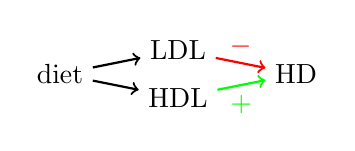
\begin{tikzpicture}
		\node (d1) at(0,0.0) {diet};
		\node (LDL) at(1.5,0.3) {LDL};
		\node (HDL) at(1.5,-0.3) {HDL};
		\node (HD) at(3,0) {HD};
		
		\draw[->,thick] (d1) -- (HDL);
		\draw[->,thick] (d1) -- (LDL);
		\draw[->,red,thick] (LDL) -- node[above,yshift=-1] {$-$} (HD);
		\draw[->,green,thick] (HDL) -- node[below] {$+$} (HD);
		\end{tikzpicture}
		\caption{}\label{fig:cholesterol:a}
	\end{subfigure}
	%
	\hfill
	%
	\begin{subfigure}{.45\linewidth}
		\center\
		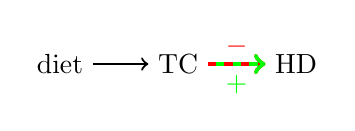
\begin{tikzpicture}
		\node (d1) at(0,0.) {diet};
		\node (LHDL) at(1.5,0) {TC};
		\node (HD) at(3,0) {HD};
		
		\draw[->,thick] (d1) -- (LHDL);
		\draw[->,red,dash pattern= on 3pt off 3pt,ultra thick] (LHDL) -- node[above,yshift=-1] {$-$} (HD);
		\draw[->,green,dash pattern= on 3pt off 3pt,dash phase=3pt,ultra thick] (LHDL) -- node[below] {$+$} (HD);
		\end{tikzpicture}
		\caption{}\label{fig:cholesterol:b}
	\end{subfigure}
	%
	\caption{Effects of cholesterol on risk of heart disease. As illustrated by~(a), the current consensus is that low-density lipoprotein (LDL) has a negative effect on heart disease (HD), while high-density lipoprotein (HDL) has a positive effect on heart disease. Considering total blood cholesterol (TC = LDL + HDL) to be a causal variable as in~(b) leads to problems: two diets promoting raised LDL levels and raised HDL levels respectively have the same effect on TC but opposite effects on heart disease. Hence different studies come to contradictory conclusions about the effect of TC on heart disease.}
	\label{fig:cholesterol}
\end{figure}


%In the following we give an example of the problems that can arise when there exists no consistent correspondence between two causal models, i.\,e.\ neither model can be viewed as an exact transformation of the other. This example falls into category (b) of the differing model levels listed above and was used by~\cite{spirtes2004causal} to illustrate problems in the causal modelling process.


Historically, the level of total blood cholesterol (TC) in a human subject was thought to be an important variable in determining their risk of developing heart disease (HD).
To investigate this, many experiments were carried out in which patients were assigned to different diets in order to raise or lower TC\@.
Conflicting evidence was found by these experiments: some found that higher TC had the effect of lowering HD, while others found the opposite \citep{truswell2010cholesterol,steinberg2011cholesterol}.

The reason for this apparent contradiction is clear with hindsight, but serves to illustrate the care that must be taken when seeking causal relations. 
The current scientific consensus is that there are two types of blood cholesterol, low-density lipoprotein (LDL) and high-density lipoprotein (HDL), which have a negative and positive effect on HD respectively (Figure \ref{fig:cholesterol:a}).
A measurement of TC is in fact a measurement of the sum of LDL and HDL.
Therefore two experiments, one raising LDL levels and the other raising HDL levels, would have the same effect on TC but opposite effects on HD (Figure \ref{fig:cholesterol:b}).

In this example, total blood cholesterol is too `coarse' a variable to have a well-defined causal relation with risk of heart disease. 
However, if it had been possible to affect only one of LDL and HDL through diet, this issue may never have been discovered:
if only HDL could be influenced by diet, the scientific consensus would be that total blood cholesterol is protective against heart disease and no contradictions would have been found.

Similarly, it is conceivable that there are in fact two different types of HDL: a more prevalent form which is protective against heart disease and one present in smaller quantities that has a detrimental impact. 
If the ratio of these two types is constant under any intervention through diet, the negative impact will always be outweighed by the positive impact and so we might never discover the detrimental subtype. 
If this were true, would the statement `increased HDL levels cause reduced risk of heart disease' be rendered false? 
Arguably it would be an oversimplification of the more complicated truth, but it would not be false in that it would correctly predict the outcome of any diet-based intervention.

This example raises two main points. The first is that in the real world, measurements or observations are always made at some level of detail or coarseness that is somewhat arbitrary.
%In the next subsection we will outline a variety of ways in which models of different levels of detail naturally arise in a variety of cases and further motivate the study of this fact in a causal setting.
The second is that whether or not a variable is `causally meaningful' is intricately connected to the interventions being considered. If we consider a coarse variable such as TC, we can consistently model causal relations if the interventions considered are sufficiently restricted, but this breaks down if the interventions are too rich. 
%In subsection ?? we will discuss how to modify the framework of SEMs to take this into account.

We elaborate on each of these points next, 
setting the stage to tackle our overarching goal of trying to answer the following questions:
If the true causal mechanisms of the world operate at a very low level of detail (e.g.~atoms), under what conditions can we speak of causal relations at higher levels (e.g.~objects)?
How can we formalise such a notion of consistent modelling in the framework of SEMs?


\subsection{Modelling at different levels of detail}\label{subsec:causality-modelling-different-levels}

All physical systems or processes in the real world are complex and can be understood at various levels of detail.
We previously discussed the example of cholesterol levels and risk of heart disease.
Although the true mechanisms by which cholesterol affects heart disease are surely very complicated -- for instance, it may be important how cholesterol is distributed throughout the body -- we sought to summarise the micro-level details into a small number of macro-level variables, the total levels of HDL and LDL.

Another example of micro-macro abstraction 
%that is more rigorously understood 
can be found in statistical physics.
A gas in a volume consists of a large number of molecules, but instead of modelling the motions of each particle individually, we may choose to consider macroscopic properties of their motions such as temperature and pressure.
As in the case of cholesterol, the decision to use such macroscopic properties may be necessitated primarily by practical considerations.
Indeed, for all but extremely simple cases, making a measurement of all the individual molecules is practically impossible and computational resources insufficient for modelling the ${\sim}10^{22}$ particles present per litre of ideal gas.
Furthermore, the decision for a macroscopic description level is also a pragmatic one: if we only wish to reason about temperature and pressure, a model of $10^{22}$ particles is ill-suited.

Statistical physics is a rigorous theory that explains how higher-level concepts such as temperature and pressure arise as statistical properties of a system of a large number of particles, justifying the use of a macro-level model as a useful transformation of the micro-level model~\citep{Balian}.
However, in many other cases where aggregate or indirect measurements of a complex system form the basis of a macroscopic description of the system (such as the cholesterol example) there is little theory to explain whether this is justified or how the micro- and macro-descriptions stand in relation to one another.
As we saw, this lack of theory occasionally leads to apparent contradictions.
%, as with the effect of total cholesterol on risk of heart disease

Due to deliberate modelling choice or the limited ability to observe a system, differing levels of model descriptions are ubiquitous and occur, amongst possibly others, in the following three settings:

\begin{itemize}[noitemsep]
	\item[(a)] Models with large numbers of variables versus models in which the `irrelevant' or unobservable variables have been marginalised out \citep{bongers2016structural}; e.\,g.\ modelling blood cholesterol levels and risk of heart disease while ignoring other blood chemicals or external factors such as stress.
	
	\item[(b)] Micro-level models versus macro-level models in which the macro-variables are aggregate features of the micro-variables \citep{simon1961aggregation,iwasaki1994causality,hoel2013quantifying,chalupka2015visual,chalupka2016multi}; e.\,g.\ instead of modelling the brain as consisting of $100$ billion neurons it can be modelled as averaged neuronal activity in distinct functional brain regions.
	
	\item[(c)] Dynamical time series models versus models of their stationary behaviour \citep{fisher1970correspondence,iwasaki1994causality,dash2001caveats,lacerda2012discovering,mooij2013ode,mooij2013cyclic}; e.\,g.\ modelling only the final ratios of reactants and products of a time evolving chemical reaction.
\end{itemize}

In each of these cases, the fine-grained model may be considered the `truth' while the coarse-grained model is a convenient abstraction.\footnote{Of coure, the fine-grained model may itself be a coarsening of an even more detailed model.} 
In the context of causal modelling, an intervention in the coarse-grained model must correspond in reality to some intervention in the fine-grained model.
Such differing model levels should be consistent with one another in the sense that they agree in their predictions of the effects of corresponding interventions. 
%In section ??, the notion of an exact transformation between two SEMs is introduced, formalising this idea of consistency of corresponding interventions, and providing a general framework to evaluate when two models can be thought of as causal descriptions of the same system.
%On a high level, if an SEM can be viewed as an exact transformation of another SEM, there is an explicit correspondence between the two models in such a way that causal reasoning on both levels is consistent.


%The particular causal models we focus on in this paper are Structural Equation Models (SEMs, Section~\ref{sec:SEMs}, Section~\ref{sec:sem-for-causal-modelling}) \citep{spirtes2000causation,pearl2009causality}.
%
%In Section~\ref{sec:sem-transformation}, we introduce the notion of an exact transformation between two SEMs, providing us with a general framework to evaluate when two models can be thought of as causal descriptions of the same system.
%An important novel idea of this paper is to explicitly make use of a natural ordering on the set of interventions.
%On a high level, if an SEM can be viewed as an exact transformation of another SEM, we are provided with an explicit correspondence between the two models in such a way that causal reasoning on both levels is consistent.
%We discuss this notion of consistency in detail in Sections~\ref{subsec:causal-interpretation-transformation} and~\ref{sec:wrong}.
%
%In Section~\ref{sec:example-transformations} we apply this mathematical framework and prove the exactness of transformations belonging to each of the three categories listed above, with practical implications for the following questions in causal modelling:
%When can we model only a subsystem of a more complex system?
%When does a micro-level system admit a causal description in terms of macro-level features?
%How do cyclic SEMs arise?
%The fact that these distinct problems can all be considered using the language of transformations between SEMs demonstrates the generality of our approach.
%We close in Section~\ref{sec:questions} with a discussion.


%It is therefore not possible to transform the model in Figure~\ref{fig:cholesterol:b} into the model in Figure~\ref{fig:cholesterol:a} without leading to conflict:
%in order to reason about the causes of HD we need to consider the variables LDL and HDL separately.

\subsection{The importance of interventions}

Recall the two models in Figure \ref{fig:cholesterol} in the cholesterol and heart disease example. 
Here, the micro-level model with variables HDL and LDL is inconsistent with the macro-level model with only the TC variable. 
The inconsistency arose because two different interventions in the mirco-level (raise HDL and raise LDL) have different effects on risk of heart disease yet map to the same intervention at the micro-level (raise TC).
This would not have been noticed had it been possible to intervene only on one of HDL and LDL through dietary means, and in this case the TC model would have been considered valid.
In other words, whether or not the two models are consistent with one another is in large part a question of which interventions in the micro-model are to be represented in the macro-model.

This is illustrative of a more general case in which the same system is modelled at two different levels of complexity: if the two models are to be considered consistent, the set of interventions modelled at the micro-level may need to be restricted, since a macro-model will generally have the capacity to express fewer interventions than a micro-model with a larger number of variables. 
This point cannot be formally expressed within the framework of classical SEMs as given by Definition \ref{def:causality-classical-sem}, since these does not specify which interventions are valid. 

Moreover, for a \emph{collection} of macro-variables to be considered a causal model consistent with a micro-level model, we must also consider compositionality, an often-overlooked natural structure present in interventions.
Given an SEM $\mathcal{M}_X$ over variables $X_1, \ldots, X_N$, the two interventions $\doop(X_i=x_i)$ and $\doop(X_j=x_j)$ for $i\not=j$  can be combined to form the intervention $\doop(X_i=x_i, X_j=x_j)$. 
This corresponds to the intuitive notion that interventions on distinct causal variables can be combined, and will be formalised by imposing a \emph{partial ordering} on the set of interventions modelled.
% in which $\doop(X_i=x_i) \leq_X \doop(X_i=x_i, X_j=x_j)$ and $\doop(X_j=x_j) \leq_X \doop(X_i=x_i, X_j=x_j)$. 
%The importance of this structure will be elaborated on in Section ??.

In summary, for macro-variables that are functions of underlying causal micro-variables to be themselves considered causal entities, it is important to consider the set of interventions being modelled and the structure exhibited by these interventions.


\section{Transformations between Structural Equation Models}\label{sec:causality-transformations-between-sems}

In this section we will first introduce an extended definition for SEMs that can capture restricted sets of interventions and the structure they exhibit.
We will then formalise a notion of \emph{exact transformations} between two SEMs. 
The idea is that if one SEM can be viewed as an exact transformation of another, they can both be viewed as consistent causal models of the same underlying system at different levels of detail. 
Elementary transformations satisfying this definition will be examined, and the main result (Theorem \ref{lemma:commuting}), which states that causal reasoning is preserved under exact transformations, is presented and discussed in detail.
Section \ref{sec:causality-causal-examples-of-transformations} presents practical examples of exact transformations covering each of the three categories of modelling abstractions discussed in Section \ref{subsec:causality-modelling-different-levels}.


\subsection{An extended definition for SEMs}

%As outlined in the last section, we first extend the usual definition of SEMs to take into account restricted sets of interventions imbued with a natural partial ordering.
The following definition extends that of the classical definition for SEMs. 
The main difference is the explicit introduction of the intervention set being modelled.
Additionally, for generality it is not assumed that the distribution $P_E$ factorises.
For convenience later on, the variables are labelled with an arbitrary index set $\indexset_X$ rather than $\{1,\ldots, N\}$, though this slight notational change has no formal impact on subsequent results.
All mentions of SEMs henceforth refer to the following definition, rather than the classical definition.

\medskip

\begin{definition}[Updated definition for SEMs]\label{def:causality-updated-sem}
	Let $\indexset_X$ be an index set.
	An SEM $\mathcal{M}_X$ over  variables ${X = (X_i : i\in\indexset_X )}$ taking value in $\mathcal{X}$ is a triple $\left(\mathcal{S}_X, \mathcal{I}_X, P_{E} \right)$ where
	\begin{itemize}[noitemsep]
		\item $\mathcal{S}_X$ is a set of structural equations $X_i = f_i\left( X_{\pa(i)} , E_i \right)\ $ for $i \in \indexset_X$;
		\item ($\mathcal{I}_X, \leq_X)$ is a subset of all perfect interventions equipped with a natural partial ordering (see below), i.\,e.\ it is an index set where each index corresponds to a particular perfect intervention on some of the $X$ variables;
		\item $P_{E}$ is a (not necessarily factorised) distribution over $E = ( E_i : i\in\indexset_X)$;
		\item with $P_E$-probability one, under any intervention ${i \in \mathcal{I}_X}$ there is a unique solution $x\in\mathcal{X}$ to the intervened structural equations. 
	\end{itemize}
\end{definition}
\medskip

As before, a perfect intervention on a single variable $\doop(X_i=x_i)$ is realised by replacing the structural equation for variable $X_i$ in $\mathcal{S}_X$ with $X_i = x_i$,
while perfect interventions on multiple variables, e.g. $\doop(X_i=x_i, X_j=x_j)$, are similarly realised by replacing the structural equations for each variable individually.
Elements of $\mathcal{I}_X$ correspond to perfectly intervening on a subset of the $X$ variables, setting them to some particular combination of values.

$\mathcal{I}_X$ is equipped with the natural partial ordering $\leq_X$ in which, for interventions ${i, j \in \mathcal{I}_X}$, ${i\leq_X j}$ if and only if $i$ intervenes on a subset of the variables that $j$ intervenes on and sets them equal to the same values as $j$.
For example, ${\doop(X_i=x_i) \leq_X \doop(X_i=x_i, X_j=x_j)}$.
Informally, this means that $j$ can be performed after $i$ without having to change or undo any of the changes to the structural equations made by $i$.
Not all pairs of elements must be comparable: for instance, if $i= \doop(X_1=x_1)$ and $j = \doop(X_2=x_2)$, then neither $i\leq_X j$ nor $j \leq_X i$. 
The observation that this structure is important and crucial use of it will be made use of in the next sections.

Aside from the treatment of interventions, Definition \ref{def:causality-updated-sem} additionally relaxes the usual assumption of acyclicity of the causal graph, 
Instead, the final condition in the definition ensures that for any intervention ${i \in \mathcal{I}_X}$, $\mathcal{M}_X$ induces a well-defined distribution over $\mathcal{X}$. 
This is always satisfied if the SEM is acyclic, but must be explicity included to also allow consideration of the cyclic case.
%This will be useful for interpreting cyclic SEMs as we will discuss later in Section ??.

The following example illustrates how SEMs are written in this notation and provides an example of a restricted set of interventions $\mathcal{I}_X$.

\medskip

\begin{example}\label{example1}
Consider the following SEM defined over the variables $\{ B_1,B_2,L \}$
%
\begin{align*}
\mathcal{S}_X = \big\{ & B_1 = E_1,\ B_2 = E_2,\ L = \operatorname{OR}(B_1,B_2,E_3) \big\} \\
%
\mathcal{I}_X = \big\{ & \nulli,\ \doop(B_1=0),\ \doop(B_2=0),\\
& \doop(B_1=0,B_2=0) \big\}, \\
%
\{ E_1,E_2,E_3 \} & \overset{\text{iid}}{\sim} \mathrm{Bernoulli}(0.5)
\end{align*}
%
where by the element $\nulli \in \mathcal{I}$ we denote the null- or empty-intervention corresponding to the unintervened SEM\@.
\end{example}

The SEM in Example~\ref{example1} could be thought of as a simple causal model of two light bulbs $B_1$ and $B_2$ and the presence of light $L$ in a room with a window.
Suppose that we have no access to the light switch and there are no curtains in the room but that we can intervene by removing the light bulbs.
We can model this restricted set of interventions by $\mathcal{I}_X$, i.\,e.\ the $\doop$-intervention on the SEM side ${\doop(B_1=0)}$  corresponds to removing the light bulb $B_1$.

The partial ordering of $\mathcal{I}_X$ corresponds to the ability to compose physical implementations of interventions. The fact that we can first remove light bulb $B_1$ (${\doop(B_1=0)}$) and then afterwards remove light bulb $B_2$ (resulting in the combined intervention ${\doop(B_1=0, B_2=0)}$)  is reflected in the partial ordering via the relation ${\doop(B_1=0) \leq_X \doop(B_1=0,B_2=0)}$.

\subsection{Partially ordered sets of distributions}

For each intervention $i \in \mathcal{I}_X$, the SEM $\mathcal{M}_X$ induces a distribution over the observable variables $X$ that we denote by $P_X^{\doop(i)}$.
Throughout, we will denote the empty- or null-intervention corresponding to the unintervened setting by $\nulli\in \mathcal{I}_X$.
For notational convenience, we will use $P_X$ and $P_X^{\doop(i)}$ interchangeably for the observational distribution.

$\mathcal{M}_X$ induces a set of joint distributions over $\mathcal{X}$, one for each intervention in $\mathcal{I}_X$, which moreover inherits the partial ordering from $\mathcal{I}_X$. 
We can write this poset of distributions as
\[\mathcal{P}_X := \left( \left\{ P_X^{\doop(i)} \enspace : \enspace i \in \mathcal{I}_X \right\}, \leq_X \right) \]
where $\leq_X$ is the partial ordering inherited from $\mathcal{I}_X$, i.\,e.\ ${P_X^{\doop(i)} \leq_X P_X^{\doop(j)} \iff i \leq_X j}$.%
%\footnote{More formally, one would need to define $\mathcal{P}_X$ to be the poset of \emph{tuples} $\left(i, P_X^{\doop(i)}\right)$ to avoid problems in the case that $P_X^{\doop(i)} = P_X^{\doop(j)}$ for some $i\not=_X j$. Doing so would not require a change to Definition **???** or affect the results of this chapter. To avoid notational burden in our exposition, we omit this treatment.}

Note that $\mathcal{P}_X$ contains all of the information in $\mathcal{M}_X$ about the different distributions implied by the SEM and, importantly, how they are related via the interventions.
For example, the distribution over the variables $X$ in the observational setting, $P_X^\nulli$, changes to $P_X^{\doop(i)}$ if we implement the intervention ${\doop(i)}$, and the partial ordering contains all information about which distributions are subsequently attainable by composing with other interventions.


\subsection{Exact transformations of SEMs}

Suppose we have a function ${\tau: \mathcal{X} \to \mathcal{Y}}$ which maps the variables of the SEM $\mathcal{M}_X$ to another space $\mathcal{Y}$.
Observe that since $X$ is a random variable, $\tau(X)$ is also a random variable.
For any distribution $P_X$ on $\mathcal{X}$ we thus obtain the distribution of the variable $\tau(X)$ on $\mathcal{Y}$ as $P_{\tau(X)} = \tau_{\#}P_X$ via the push-forward measure. 

%\todo{Possibly change push-forward notation to use hash. Check compatibility with WAE section.}

In particular, for each intervention $i \in \mathcal{I}_X$ we can define the induced distribution $P_{\tau(X)}^{i} = \tau_{\#}P_X^{\doop(i)}$.
We can write the poset of distributions on $\mathcal{Y}$ that are induced by the original SEM $\mathcal{M}_X$ and the transformation $\tau$ as
\[\mathcal{P}_{\tau(X)} := \left( \left\{ P_{\tau(X)}^{i} \enspace : \enspace i \in \mathcal{I}_X \right\}, \leq_X \right) \]
where $\leq_X$ is the partial ordering inherited from $\mathcal{P}_X$ (in turn inherited from $\mathcal{I}_X$).

$\mathcal{P}_{\tau(X)}$ is just a structured collection of distributions over $\mathcal{Y}$, indexed by interventions $\mathcal{I}_X$ on the $\mathcal{X}$-level; importantly, the indices are \emph{not} interventions on the $\mathcal{Y}$-level.



Although $\mathcal{P}_{\tau(X)}$ is a poset of distributions over $\mathcal{Y}$, there does not necessarily exist an SEM $\mathcal{M}_Y$ over $\mathcal{Y}$ that implies it.
For instance, if there is some intervention ${i \in \mathcal{I}_X \setminus \{ \nulli \}}$ such that none of the variables $Y_i$ is constant under the distribution $P_{\tau(X)}^{i}$, then $P_{\tau(X)}^{i}$ could not possibly be expressed as arising from a $\doop$-intervention $j\in \mathcal{I}_Y \setminus \{\nulli\}$ in any SEM over~$\mathcal{Y}$, an issue that is studied in detail by \cite{eberhardt2016green}.

The case in which there \emph{does} exist an SEM $\mathcal{M}_Y$ that implies $\mathcal{P}_{\tau(X)}$ is special, motivating our main definition.

\medskip

\begin{definition}[Exact Transformations between SEMs]\label{def:exacttrafos}
Let $\mathcal{M}_X$ and $\mathcal{M}_Y$ be SEMs and $\tau: \mathcal{X} \to \mathcal{Y}$ be a function.
We say $\mathcal{M}_Y$ is an \emph{exact}  $\tau$-transformation of $\mathcal{M}_X$ if there exists a \emph{surjective order-preserving} map $\omega:\mathcal{I}_X\rightarrow \mathcal{I}_Y$ such that
\[ P_{\tau(X)}^{i} = P_Y^{\doop(\omega(i))} \quad \forall i \in \mathcal{I}_X \]
where $P_{\tau(X)}^{i}$ is the distribution of the $\mathcal{Y}$-valued random variable $\tau(X)$ with $X \sim P_X^{\doop(i)}$.
\end{definition}

Order-preserving means that ${i \leq_X j \implies \omega(i) \leq_Y \omega(j)}$.
It is important that the converse need not in general hold as this would imply that $\omega$ is injective,%
\footnote{Since ${\omega(i)=\omega(j) \iff \left(\omega(i) \leq_Y \omega(j)\right) \land \left(\omega(j) \leq_Y \omega(i)\right)}$, which, if the converse held, would imply that $\left(i \leq_X j\right) \land \left(j \leq_X i\right)$, which is equivalent to $i=j$.}
and hence also bijective.
This would constrain the ways in which $\mathcal{M}_Y$ can be `simpler' than $\mathcal{M}_X$.\footnote{For instance, if it were necessary that $\omega$ be bijective, Theorems~\ref{theorem:childless} and \ref{theorem:micro-macro} would not hold.}
That $\omega$ is surjective ensures that for any $\doop$-intervention $j \in \mathcal{I}_Y$ on $\mathcal{M}_Y$ there is at least one corresponding intervention on the $\mathcal{M}_X$ level, namely an element of $\omega^{-1}(\{j\}) \subseteq \mathcal{I}_X$.

The following two results give elementary properties of exact transformations following immediately from the definition.
\medskip

\begin{lemma}\label{lemma:elementary}
The identity mapping and permuting the labels of variables are both exact transformations.
That is, if $\mathcal{M}_X$ is an SEM and $\pi:\mathbb{I}_X \to \mathbb{I}_X$ is a bijection then the transformation
\begin{align*}
\tau:\mathcal{X}&\to\mathcal{Y}\\
(x_i:i\in\mathbb{I}_X) &\mapsto (x_{\pi(i)}:i\in\mathbb{I}_X)
\end{align*}
naturally gives rise to an SEM $\mathcal{M}_Y$ that is an exact $\tau$-transformation of $\mathcal{M}_X$, corresponding to relabelling the variables.
\end{lemma}

\begin{proof}
Consider the SEM $\mathcal{M}_Y$ obtained from $\mathcal{M}_X$ by replacing, for all $i\in\mathbb{I}_X$, any occurrence of $X_i$ in the structural equations $\mathcal{S}_X$ and interventions $\mathcal{I}_X$ by $Y_{\pi(i)}$ and leaving the distribution over the exogenous variables unchanged. Denote by $\omega$ the corresponding mapping on interventions obtained by replacing $X_i$ with $Y_{\pi(i)}$.
\end{proof}

This is a good sanity check; it would be problematic if this were not the case and the labelling of our variables mattered. Similarly, compositions of exact transformations are also exact.

\medskip

\begin{lemma}[Transitivity of exact transformations]\label{theorem:transitivity}
    If $\mathcal{M}_Z$ is an exact $\tau_{ZY}$-transformation of $\mathcal{M}_Y$ and $\mathcal{M}_Y$ is an exact $\tau_{YX}$-transformation of $\mathcal{M}_X$, then $\mathcal{M}_Z$ is an exact $(\tau_{ZY}\circ\tau_{YX})$-transformation of $\mathcal{M}_X$.
\end{lemma}

\begin{proof}
    Let $\omega_{ZY}:\mathcal{I}_Y \to \mathcal{I}_Z$ and $\omega_{YX}:\mathcal{I}_X \to \mathcal{I}_Y$ be the mappings between interventions corresponding to the exact transformations $\tau_{ZY}$ and $\tau_{YX}$ respectively and define $\omega_{ZX} = \omega_{ZY}\circ\omega_{YX}:\mathcal{I}_X \to \mathcal{I}_Z$.
    Then $\omega_{ZX}$ is surjective and order-preserving since both $\omega_{ZY}$ and $\omega_{YX}$ are surjective and order-preserving.
    Since $\tau_{ZY}$ and $\tau_{YX}$ are exact it follows that for all $i\in\mathcal{I}_X$.
    \begin{align*}
        P^{i}_{\tau_{ZX}(X)}
        =
        P^{ \omega_{ZY}(\omega_{YX}(i))}_{\tau_{ZY}(\tau_{YX}(X))}
        =
        P^{\doop(\omega_{ZX}(i))}_{Z}
    \end{align*}
    i.\,e.\ $\mathcal{M}_Z$ is an $\tau_{ZX}$-exact transformation of $\mathcal{M}_X$.
\end{proof}



\subsection{Causal interpretation of exact transformations}
The notion of an exact transformation between SEMs was motivated by the desire to analyse the correspondence between two causal models describing the same system at different levels of detail.
The purpose of this section is to show that if one SEM can be viewed as an exact transformation of the other, then both can sensibly be thought of as causal models of the same system. 
The main technical result is the following theorem.

\medskip

\begin{theorem}[Causal consistency under exact transformations]\label{lemma:commuting}
Suppose that  $\mathcal{M}_Y$ is an exact $\tau$-transformation of $\mathcal{M}_X$ and $\omega$ is a corresponding surjective order-preserving mapping between interventions. Let $i,j \in \mathcal{I}_X$ be interventions such that $i\leq_X j$.
Then the following diagram commutes:
\begin{center}
\begin{tikzpicture}[thick, every node/.style = {circle, minimum size=.5cm}]

{
  \node[draw=none](Px) {$P_X$};
  \node[draw=none, right of=Px, xshift=2cm](PxInt) {$P_X^{\doop(i)}$};
  \node[draw=none, right of=PxInt, xshift=2cm](PxInt2) {$P_X^{\doop(j)}$};

  \node[draw=none, below of=Px, yshift=-1.5cm](Py) {$P_Y$};
  \node[draw=none, right of=Py, xshift=2cm](PyInt) {$P_Y^{\doop(\omega(i))}$};
  \node[draw=none, right of=PyInt, xshift=2cm](PyInt2) {$P_Y^{\doop(\omega(j))}$};

  \draw[-{Latex[length=2mm,width=2mm]}](Px)--(Py);
  \draw[-{Latex[length=2mm,width=2mm]}](Px)--(PxInt);
  \draw[-{Latex[length=2mm,width=2mm]}](Py)--(PyInt);
  \draw[-{Latex[length=2mm,width=2mm]}](PxInt)--(PyInt);
  \draw[-{Latex[length=2mm,width=2mm]}](PxInt)--(PxInt2);
  \draw[-{Latex[length=2mm,width=2mm]}](PyInt)--(PyInt2);
  \draw[-{Latex[length=2mm,width=2mm]}](PxInt2)--(PyInt2);

  \node[draw=none, yshift=0.5cm](xInt) at ($(Px)!0.5!(PxInt)$){$\doop(i)$};
  \node[draw=none, yshift=0.5cm](xInt2) at ($(PxInt)!0.5!(PxInt2)$){$\doop(j)$};
  \node[draw=none, yshift=0.5cm](yInt) at ($(Py)!0.5!(PyInt)$){$\doop(\omega(i))$};
  \node[draw=none, yshift=0.5cm](yInt2) at ($(PyInt)!0.5!(PyInt2)$){$\doop(\omega(j))$};
  \node[draw=none, xshift=-0.5cm](tau) at ($(Px)!0.5!(Py)$){$\tau$};
  \node[draw=none, xshift=0.5cm](tauInt) at ($(PxInt)!0.5!(PyInt)$){$\tau$};
  \node[draw=none, xshift=0.5cm](tauInt2) at ($(PxInt2)!0.5!(PyInt2)$){$\tau$};
}
\end{tikzpicture}
\end{center}
\end{theorem}

\begin{proof}
Let $i,j\in\mathcal{I}_X$ be interventions with $i\leq_X j$.
The commutativity of the left square of the diagram follows immediately from the definition of an exact transformation.
It remains to be shown that the right square of the diagram commutes.
By definition we have that $\tau_{\#}P_X^{\doop(i)} = P_Y^{\doop(\omega(i))}$ and $\tau_{\#}P_X^{\doop(j)} = P_Y^{\doop(\omega(j))}$.
Thus, we only have to show that ${P_Y^{\doop(\omega(i))} \leq_Y P_Y^{\doop(\omega(j))}}$ as elements of $\mathcal{P}_Y$, i.\,e.\ that the arrow ${P_Y^{\doop(\omega(i))} \xrightarrow{\doop(\omega(j))} P_Y^{\doop(\omega(j))}}$ exists.
This follows from the order-preservingness of $\omega$.
\end{proof}

Suppose now that $\mathcal{M}_X$ is a causal model that is taken to be in some sense `true'.
We will examine the implications of another SEM $\mathcal{M}_Y$ being an exact $\tau$-transformation of $\mathcal{M}_X$ with corresponding intervention map $\omega$.

Surjectivity of $\omega$ ensures that any intervention in $\mathcal{I}_Y$ can be viewed as an $\mathcal{M}_Y$-level representative of some intervention on the $\mathcal{M}_X$-level. Consequently, if $\doop$-interventions on the $\mathcal{M}_X$-level are in correspondence with physical implementations, then surjectivity of $\omega$ ensures that $\doop$-interventions on the $\mathcal{M}_Y$-level have at least one corresponding physical implementation.
Thus, if $\mathcal{M}_X$ is physically grounded, so is $\mathcal{M}_Y$.

Commutativity of the left hand part of the diagram ensures that the effects of interventions are consistently modelled by $\mathcal{M}_X$ and $\mathcal{M}_Y$.
Suppose we want to reason about the effects on the $\mathcal{M}_Y$-level caused by the intervention $j \in \mathcal{I}_Y$.
For example, we may wish to reason about how the temperature and pressure of a volume of gaseous particles is affected by being heated.
We could perform this reasoning by considering any corresponding $\mathcal{M}_X$-level intervention $i \in \omega^{-1}(\{j\})$ and considering the distribution this implies over $\mathcal{Y}$ via $\tau$.
In our example, this would correspond to considering how heating the volume of gas could be modelled by changing the motions of all the gaseous particles and then computing the temperature and pressure of the volume of particles.
Commutativity of the left hand part of the diagram implies that $\mathcal{M}_X$ and $\mathcal{M}_Y$ are consistent in the sense that $\mathcal{M}_Y$ allows us to immediately reason about the effect of the intervention $j\in\mathcal{I}_Y$ while being equivalent to performing the steps above.
That is, we can reason directly about temperature and pressure when heating a volume of gas without having to perform the intermediate steps that involve the microscopic description of the system.

Commutativity of the right hand side of the diagram ensures that once an intervention that fixes a subset of the variables has been performed, we can still consistently reason about the effects of further interventions on the remaining variables in $\mathcal{M}_X$ and $\mathcal{M}_Y$.
Furthermore, it ensures that compositionality of $\doop$-interventions on the $\mathcal{M}_X$-level carries over to the $\mathcal{M}_Y$-level.
That is, if the intervention $j$ on the $\mathcal{M}_X$-level can be performed additionally to the intervention $i$ in $\mathcal{M}_X$ (i.\,e.\ $i\leq_X j$), then the same is true of their representations in $\mathcal{M}_Y$.

If $\mathcal{M}_X$ and $\mathcal{M}_Y$ are models of the same system and it has been established that $\mathcal{M}_Y$ is an exact $\tau$-transformation of $\mathcal{M}_X$ for some mapping $\tau$, then the commutativity of the whole diagram in Theorem~\ref{lemma:commuting} ensures that they are causally consistent with one another in the sense described in the preceding paragraphs.
If we wish to reason about the effects of interventions on the $\mathcal{Y}$-variables then it suffices to use the model $\mathcal{M}_Y$, rather than the (possibly more complex) model $\mathcal{M}_X$.
In particular, this means that we can view the $\mathcal{Y}$-variables as causal entities, rather than only functions of underlying `truly' causal entities.
Only if this is the case, causal statements such as `raising temperature increases pressure' or `LDL causes heart disease' are meaningful.

\subsection{What can go wrong when a transformation is not exact?}\label{sec:wrong}

In the previous section it was argued that Definition \ref{def:exacttrafos} of exact transformations between SEMs is a sensible formalisation of causal consistency.
This section provides intuition for why weakening the conditions of the definition would be problematic.
Particular focus is paid to the requirement that $\omega$ be order-preserving, which is one of the core ideas of this work.

The requirement that $\omega$ be surjective is, as discussed above, required so that all interventions on the $\mathcal{M}_Y$-level have a corresponding intervention on the $\mathcal{M}_X$-level.
If it were only required that $\omega$ be surjective (but not order-preserving), the observational distribution of $\mathcal{M}_X$ might be mapped to an interventional distribution of $\mathcal{M}_Y$, as illustrated by the following example, illustrated in Figure~\ref{fig:wrong-example}.

\begin{figure}
\begin{subfigure}{.45\linewidth}
\center\
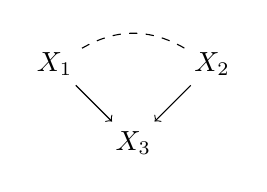
\begin{tikzpicture}
\node (x1) at(0,0) {$X_1$};
\node (x2) at(2,0) {$X_2$};
\node (x3) at(1,-1) {$X_3$};

\draw[->] (x1) -- (x3);
\draw[->] (x2) -- (x3);
\draw[dashed] (x1) to [bend left] (x2);
\end{tikzpicture}
\caption{SEM $\mathcal{M}_X$}
\end{subfigure}
%
\hfill
%
\begin{subfigure}{.45\linewidth}
\center\
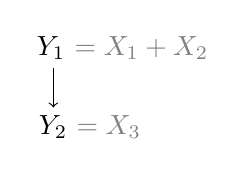
\begin{tikzpicture}
\node (y1) at(0,0) {$Y_1\ {\color{gray}= X_1+X_2}$};
\node (y2) at(-.415,-1) {$Y_2\ {\color{gray}= X_3}$};

\draw[->] (-.88,-.25) -- (-.88,-.75);
\end{tikzpicture}
\caption{SEM $\mathcal{M}_Y$}
\end{subfigure}
%
\caption{Graphical illustration of parent-child relationships for the examples in Section~\ref{sec:wrong}. The micro-level model $\mathcal{M}_X$ depicted in (a) is to be transformed into the macro-level model $\mathcal{M}_Y$ depicted in (b) which is a coarser descriptions as in it only considers the sum of $X_1$ and $X_2$. In Section~\ref{sec:wrong} we give examples of what can go wrong if the transformation is not exact.}
\label{fig:wrong-example}
\end{figure}

\medskip

\begin{example}\label{example:wrong1}
Consider the SEM $\mathcal{M}_X=\{\mathcal{S}_X , \mathcal{I}_X, \mathbb{P}_E\}$ over $\mathcal{X}=\mathbb{R}^3$ where
%
\begin{align*}
\mathcal{S}_X = \big\{ & X_1 = E_1,\ X_2 = E_2,\ X_3 = X_1 + X_2 + E_3 \big\} \\
%
\mathcal{I}_X = \big\{ & \nulli,\ \doop(X_2=0),\ \doop(X_1=0,\, X_2=0)\big\}, \\
%
E_1 & \sim \mathbb{P}_{E_1},\ \,  E_2 = - E_1, \  \, E_3 \sim \mathbb{P}_{E_3}
\end{align*}
%
where $\mathbb{P}_{E_1}$ and $\mathbb{P}_{E_3}$ are arbitrary distributions.
Let ${\tau:\mathcal{X}\to\mathcal{Y}=\mathbb{R}^2}$ be the mapping such that
\begin{align*}
\tau\begin{pmatrix} x_1, x_2, x_3 \end{pmatrix}
= \begin{pmatrix} y_1, y_2\end{pmatrix}
= \begin{pmatrix} x_1 + x_2, x_3\end{pmatrix}
\end{align*}
%
Let $\mathcal{M}_Y =\{\mathcal{S}_Y , \mathcal{I}_Y, \mathbb{P}_F\}$ be an SEM over $\mathcal{Y}$ with
%
\begin{align*}
\mathcal{S}_Y = \big\{ & Y_1 = F_1,\ Y_2 = Y_1 + F_2 \big\} \\
%
\mathcal{I}_Y = \big\{ & \nulli,\ \doop(Y_1=0) \big\}, \\
%
F_1 \sim \mathbb{P}_{E_1},&  \  \, F_2 \sim \mathbb{P}_{E_3}
\end{align*}
%
Let ${\omega:\mathcal{I}_X \to \mathcal{I}_Y}$ be defined by
%
\begin{align*}
\omega: \begin{cases}
\nulli &\mapsto \doop(Y_1=0) \\
\doop(X_2=0) &\mapsto \nulli \\
\doop(X_1=0,\, X_2=0) &\mapsto \doop(Y_1=0) \\
\end{cases}
\end{align*}
%
Then it is true that ${\mathbb{P}_{\tau(X)}^{i} = \mathbb{P}_Y^{\doop(\omega(i))}}$ for all  ${i \in \mathcal{I}_X }$, while $\omega$ is not order-preserving and $\omega(\nulli)\not = \nulli$.
\end{example}

If the SEMs in the above example were used to model the same system, it would be problematic that the observational setting of $\mathcal{M}_X$---a description of the system when not having physically performed any intervention---would correspond to an interventional setting in $\mathcal{M}_Y$, conversely suggesting that the system \emph{had} been intervened upon.

To avoid the above conflict, it could be demanded in addition to surjectivity that $\omega$ map the null intervention of $\mathcal{M}_X$ to the null intervention of $\mathcal{M}_Y$.
This additional assumption would ensure commutativity of the left-hand part of the diagram in Theorem~\ref{lemma:commuting}.
However, as the following example shows, this would not ensure that the right-hand part of the diagram commutes for all pairs of interventions ${i \leq_X j}$, since in this case the arrow from $\mathbb{P}_Y^{\doop(\omega(i))}$ to $\mathbb{P}_Y^{\doop(\omega(j))}$ may not exist.\footnote{By definition of the poset $\mathcal{P}_Y$, this arrow exists if and only if $\omega(i) \leq_Y \omega(j)$.}

\medskip

\begin{example}\label{example:wrong2}
Let $\mathcal{X},\mathcal{Y}$ and $\tau$ be as in Example~\ref{example:wrong1}. Consider the SEM $\mathcal{M}_X=\{\mathcal{S}_X , \mathcal{I}_X, \mathbb{P}_E\}$ where
%
\begin{align*}
\mathcal{S}_X = \big\{ & X_1 = E_1,\ X_2 = E_2, \ X_3 = X_1 + X_2 + E_3 \big\} \\
%
\mathcal{I}_X = \big\{ & \nulli,\ \doop(X_2=0),\ \doop(X_1=0,\, X_2=0)\big\}, \\
%
E_1 & = 1,\ \,  E_2 \sim \mathbb{P}_{E_2}, \  \, E_3 \sim \mathbb{P}_{E_3}
\end{align*}
%
where $\mathbb{P}_{E_2}$ and $\mathbb{P}_{E_3}$ are arbitrary distributions.
%
Let $\mathcal{M}_Y =\{\mathcal{S}_Y , \mathcal{I}_Y, \mathbb{P}_F\}$ be the SEM over $\mathcal{Y}$ with
%
\begin{align*}
\mathcal{S}_Y = \big\{ & Y_1 =1+ F_1,\ Y_2 = Y_1 + F_2 \big\} \\
%
\mathcal{I}_Y = \big\{ & \nulli,\ \doop(Y_1=0),\ \doop(Y_1=1) \big\}, \\
%
F_1 &\sim \mathbb{P}_{E_2},  \  \, F_2 \sim \mathbb{P}_{E_3}
\end{align*}
%
Let ${\omega:\mathcal{I}_X \to \mathcal{I}_Y}$ be defined by
%
\begin{align*}
\omega: \begin{cases}
\nulli &\mapsto \nulli  \\
\doop(X_2=0) &\mapsto \doop(Y_1=1) \\
\doop(X_1=0,\, X_2=0) &\mapsto \doop(Y_1=0) \\
\end{cases}
\end{align*}
%
Then it is true that ${\mathbb{P}_{\tau(X)}^{i} = \mathbb{P}_Y^{\doop(\omega(i))}}$ for all ${i \in \mathcal{I}_X}$ and $\omega(\nulli)=\nulli$, although $\omega$ is not order-preserving.
\end{example}

If the above SEMs were used as models of the same system, they would not suffer from the problem illustrated in Example~\ref{example:wrong1}.
Suppose now, however, that we have performed the intervention $\doop(X_2=0)$ in $\mathcal{M}_X$, corresponding to the intervention $\doop(Y_1=1)$ in $\mathcal{M}_Y$.
If we wish to reason about the effect of the intervention $\doop(X_1=0,\, X_2=0)$ in $\mathcal{M}_X$, we run into a problem.
$\mathcal{M}_X$ suggests that $\doop(X_1=0,\, X_2=0)$ could be implemented by performing an additional action on top of $\doop(X_2=0)$.
In contrast, $\mathcal{M}_Y$ suggests that implementing the corresponding intervention $\doop(Y_1=0)$ would conflict with the already performed intervention $\doop(Y_1=1)$.
The requirement that $\omega$ be order-preserving rules this pathology out. 

\section{Examples of transformations}\label{sec:causality-causal-examples-of-transformations}

The problem of modelling at multiple levels of complexity was motivated in Section \ref{subsec:causality-modelling-different-levels} by listing three settings in which differing model levels naturally occur.
Having now introduced the notion of an exact transformation between SEMs, we provide in this section examples of exact transformations falling into each of these categories.
%The fact that a single framework can be used to draw an explicit correspondence between differing model levels in each of these settings demonstrates the generality of our framework.

Observe that in each of the following examples, the particular set of interventions considered is important. If we were to allow larger sets of interventions $\mathcal{I}_X$ in the SEM $\mathcal{M}_X$, the transformations given would not be exact. This highlights the importance to the causal modelling process of carefully considering the set of interventions. All proofs are found in Appendix \ref{chapter:appendix-causality}.






\subsection{Marginalisation of variables}\label{sec:basic_trafos}

In the following two theorems it is shown that the marginalisation of childless or non-intervened variables is an exact transformation, illustrated in Figure~\ref{fig:SEM_marginalisation}.
That is, an SEM can be simplified into an SEM by marginalising out variables of either of these types without losing any causal content concerning the remaining variables.

Thus if the SEM $\mathcal{M}_Y$ can be obtained from another SEM $\mathcal{M}_X$ by successively performing the operations in the following theorems, then $\mathcal{M}_Y$ is an exact transformation of $\mathcal{M}_X$ and hence the two models are causally consistent.
This formally explains why we can sensibly consider causal models that focus on a subsystem $\mathcal{M}_Y$ of a more complex system $\mathcal{M}_X$.
%For a measure-theoretic treatment of marginalisation in SEMs, see~\cite{bongers2016structural}.

\begin{figure}
\center\
%
\begin{tikzpicture}

\node[keep] (X1) at(0,0) {$X_1$};
\node[keep] (X2) at(1.5,1.5) {$X_2$};
\node[keep] (X3) at(3,0) {$X_3$};

\node[drop1] (d1) at(4.5,.25) {};
\node[drop1] (d2) at(4.5,1.25) {};
\node[drop1] (d3) at(5,.75) {};

\draw[->,docolour] (X3) -- (d1);
\draw[->,docolour] (X2) -- (d2);
\draw[->,docolour] (d2) -- (d1);
\draw[->,docolour] (d1) -- (d3);
\draw[->,docolour] (d2) -- (d3);
\draw[->,docolour,dashed] (d1) -- (5,0);
\draw[->,docolour,dashed] (d2) -- (5,1.5);

\node[drop2a] (i12) at(.75,.75) {};
\node[drop2a] (i23) at(2.25,.75) {};
\node[drop2a] (i13a) at(1,0) {};
\node[drop2a] (i13b) at(2,0) {};

\draw[->] (X1) -- (i12) -- (X2);
\draw[->] (X2) -- (i23) -- (X3);
\draw[->] (X1) -- (i13a) -- (i13b) -- (X3);
\draw[->,docolour,dashed] (i13a) -- (1.25,-1);

\node[drop2b] (n1) at(-1.5,.5) {};
\node[drop2b] (n2) at(-1,1.5) {};
\node[drop2b] (n3) at(-1.75,1.25) {};

\draw[->,docolour] (n1) -- (X1);
\draw[->,docolour] (n3) -- (n1);
\draw[->,docolour] (n1) -- (n2);
\draw[->,docolour] (n3) -- (n2);
\draw[->,docolour,dashed] (-1.75,0) -- (n1);
\draw[->,docolour,dashed] (-1.75,2) -- (n2);
\draw[->,docolour,dashed] (-1,-.25) -- (X1);
\draw[->,docolour,dashed] (-.5,2.5) -- (X2);

\draw[dotted] (-.75,2.25) -- (3.75,2.25) -- (3.75,-.75) -- (-.75,-.75) -- (-.75,2.25);
\node (label) at(1.5,2.5) {subsystem $\mathcal{M}_Y$};
\node (label2) at(-1.75,-.75) {$\mathcal{M}_X$};

\end{tikzpicture}
%
\caption{Suppose that there is a complex model $\mathcal{M}_X$ but that we only wish to model the distribution over $X_1,X_2,X_3$ and how it changes under some interventions on $X_1,X_2,X_3$.
By Theorem~\ref{theorem:childless}, we can ignore downstream effects (\dropNode{drop1}) after grouping them together as one multivariate variable and by Theorem~\ref{theorem:never_intervened} we can ignore intermediate steps of complex mechanisms (\dropNode{drop2a}) and treat upstream causes as noise fluctuations (\dropNode{drop2b}).
That is, we can exactly transform the complex SEM $\mathcal{M}_X$ into a simpler model $\mathcal{M}_Y$ by marginalisation.
}
\label{fig:SEM_marginalisation}
\end{figure}

\medskip

\begin{theorem}[Marginalisation of childless variables]\label{theorem:childless}
Let $\mathcal{M}_X=(\mathcal{S}_X,\mathcal{I}_X,\mathbb{P}_E)$ be an SEM and suppose that ${\mathbb{I}_Z\subset\mathbb{I}_X}$ is a set of indices of variables with no children, i.\,e.\ if $i\in\mathbb{I}_Z$ then $X_i$ does not appear in the right-hand side of any structural equation in $\mathcal{S}_X$.
Let $\mathcal{Y}$ be the set in which $Y = \left( X_i: i\in\mathbb{I}_X\setminus \mathbb{I}_Z \right)$ takes value.
Then the transformation $\tau: \mathcal{X} \to \mathcal{Y}$ mapping
\begin{align*}
   \tau: \left( x_i: i\in\mathbb{I}_X \right) = x &\mapsto y = \left( x_i: i\in\mathbb{I}_X\setminus \mathbb{I}_Z \right)
\end{align*}
naturally gives rise to an SEM $\mathcal{M}_Y$ that is an exact $\tau$-transformation of $\mathcal{M}_X$, corresponding to marginalising out the childless variables $X_i$ for $i\in\mathbb{I}_Z$.
\end{theorem}



\medskip


\begin{theorem}[Marginalisation of non-intervened variables]\label{theorem:never_intervened}
Let $\mathcal{M}_X=(\mathcal{S}_X,\mathcal{I}_X,\mathbb{P}_E)$ be an \emph{acyclic} SEM and suppose that ${\mathbb{I}_Z\subset\mathbb{I}_X}$ is a set of indices of variables that are not intervened upon by any intervention $i\in\mathcal{I}_X$.
Let $\mathcal{Y}$ be the set in which $Y = \left( X_i: i\in\mathbb{I}_X\setminus \mathbb{I}_Z \right)$ takes value.
Then the transformation $\tau: \mathcal{X} \to \mathcal{Y}$ mapping
\begin{align*}
   \tau: \left( x_i: i\in\mathbb{I}_X \right) = x &\mapsto y = \left( x_i: i\in\mathbb{I}_X\setminus \mathbb{I}_Z \right)
\end{align*}
naturally gives rise to an SEM $\mathcal{M}_Y$ that is an exact $\tau$-transformation of $\mathcal{M}_X$, corresponding to marginalising out the never-intervened-upon variables $X_i$ for $i\in\mathbb{I}_Z$.
\end{theorem}

\medskip

The assumption of acyclicity made in Theorem~\ref{theorem:never_intervened} can be relaxed to allow marginalisation of non-intervened variables in cyclic SEMs, at the expense of extra technical conditions; see Section~3 of \cite{bongers2016structural}.

Recall that Definition \ref{def:causality-updated-sem} does not require that the exogenous $E$-variables of a SEM be independent. 
Theorem~\ref{theorem:never_intervened} would not hold if this restriction were made (which is usually the case in the literature); marginalising out a common parent node will in general result in its children having dependent exogenous variables.

\subsection{Micro- to macro-level}\label{subsection:micromacro}

Transformations from micro- to macro-levels may arise in situations in which the micro-level variables can be observed via a `coarse' measurement device, represented by the function $\tau$, e.\,g.\ we can use a thermometer to measure the temperature of a gas, but not the motions of the individual particles. They may also arise due to deliberate modelling choice when we wish to describe a system using higher level features, e.\,g.\ viewing the motor cortex as a single entity responsible for movements, rather than as a collection of individual neurons.

In such situations, our framework of exact transformations allows one to investigate whether such a macro-level model admits a causal interpretation. The following theorem provides an exact transformation between a micro-level model $\mathcal{M}_X$ and a macro-level model $\mathcal{M}_Y$ in which the variables are aggregate features of variables in $\mathcal{M}_X$ obtained by averaging (cf.\ Figure~\ref{fig:micro_macro}).

\medskip

\begin{theorem}[Micro- to macro-level]\label{theorem:micro-macro}
Let ${\mathcal{M}_X = \left(\mathcal{S}_X, \mathcal{I}_X, \mathbb{P}_{E,F} \right)}$ be a linear SEM over the variables ${W=\left( W_i \: : \: 1\leq  i \leq n \right)}$ and ${Z=\left( Z_i \: : \: 1\leq  i \leq m \right)}$ with
%
\begin{align*}
\mathcal{S}_X &= \left\lbrace W_i = E_i \:  : \: 1 \leq i \leq n  \right\rbrace \\
& \quad \ \  \cup \left\lbrace Z_i = \sum_{j=1}^n A_{ij}W_j  + F_{i} \:  : \: 1\leq i \leq m \right\rbrace \\
%
\mathcal{I}_X &= \Big{\{} \nulli, \ \doop(W= w), \ \doop(Z= z), \\
& \qquad\ \doop(W= w, Z= z ) :   w \in \mathbb{R}^{n}, \, z \in \mathbb{R}^m \Big{\}}
%
\end{align*}
%
and $(E,F)  \sim \mathbb{P}$ where $\mathbb{P}$ is any distribution over $\mathbb{R}^{n+m}$ and $A$ is a matrix.

Assume that there exists an $a\in \mathbb{R}$ such that each column of $A$ sums to $a$. Consider the following transformation that averages the $W$ and $Z$ variables:
%
\begin{align*}
\tau : \mathcal{X} &\rightarrow \mathcal{Y} = \mathbb{R}^2 \\
\begin{pmatrix} W \\ Z \end{pmatrix} &\mapsto \begin{pmatrix} \widehat{W} \\ \widehat{Z} \end{pmatrix} = \begin{pmatrix} \frac{1}{n}\sum_{i=1}^n W_i \\ \frac{1}{m}\sum_{j=1}^m Z_j  \end{pmatrix}
\end{align*}
%
Further, let $\mathcal{M}_Y = \left(\mathcal{S}_Y, \mathcal{I}_Y, \mathbb{P}_{\widehat{E},\widehat{F}} \right)$ over the variables ${\left\lbrace \widehat{W}, \widehat{Z} \right\rbrace}$ be an SEM with
%
\begin{align*}
\mathcal{S}_Y &= \Big\lbrace \widehat{W} = \widehat{E}, \ \widehat{Z} = \frac{a}{m}\widehat{W} + \widehat{F} \Big\rbrace \\
%
\mathcal{I}_Y &= \Big{\{} \nulli,\ \doop(\widehat{W}= \widehat{w}), \ \doop(\widehat{Z}= \widehat{z}), \\
& \qquad\ \doop(\widehat{W}= \widehat{w}, \widehat{Z}= \widehat{z} ) :   \widehat{w} \in \mathbb{R}, \, \widehat{z} \in \mathbb{R} \Big{\}} \\
%
\widehat{E}  & \sim \frac{1}{n}\sum_{i=1}^{n} E_i, \quad
\widehat{F}  \sim \frac{1}{m}\sum_{i=1}^{m} F_i
\end{align*}

Then $\mathcal{M}_Y$ is an exact $\tau$-transformation of $\mathcal{M}_X$.
\end{theorem}

\medskip


\begin{figure}
\center\
%
\begin{tikzpicture}
\node[ellipse, draw,blue, fill=blue!20, minimum width=3.2cm, minimum height=1.2cm,rotate=-20] (e1) at (0,0) {};
\node[ellipse, draw,blue, fill=blue!20, minimum width=3cm, minimum height=1cm,rotate=40] (e2) at (4,0) {};


\node[micro] (X1) at(-.7,.1) {};
\node[micro] (X2) at(0.1,0.3) {};
\node[micro] (X3) at(.3,-0.4) {};
\node[micro] (X4) at(.8,-0.1) {};

\node[micro] (Z1) at(4.1,.3) {};
\node[micro] (Z2) at(3.8,-.2) {};
\node[micro] (Z3) at(3.2,-.7) {};

\draw[->,docolour] (X1) -- (Z1);
\draw[->,docolour] (X1) -- (Z2);
\draw[->,docolour] (X2) -- (Z1);
\draw[->,docolour] (X2) -- (Z2);
\draw[->,docolour] (X3) -- (Z1);
\draw[->,docolour] (X3) -- (Z2);
\draw[->,docolour] (X3) -- (Z3);
\draw[->,docolour] (X4) -- (Z3);

\node[blue] (label1) at(.45,1.7) {$\widehat{W}$};
\node[blue] (label2) at(3.7,1.7) {$\widehat{Z}$};

\node (MY) at(-2,1.7) {$\mathcal{M}_Y$:};
\node (MX) at(-2,0) {$\mathcal{M}_X$:};

\begin{pgfonlayer}{background}
\shade[bottom color=white,top color=blue!50!white,shading angle=160] (e1.0)--(label1.275)--(label1.245)--(e1.180)--cycle;
\shade[bottom color=white,top color=blue!50!white,shading angle=200] (e2.0)--(label2.285)--(label2.255)--(e2.180)--cycle;
\end{pgfonlayer}

\draw[->,blue,thick] (label1) -- (label2) ;

\end{tikzpicture}
%
\caption{ An illustration of the setting considered in Theorem~\ref{theorem:micro-macro}. The micro-variables $W_1,\ldots,W_n$ and $Z_1,\ldots,Z_m$ in the SEM $\mathcal{M}_X$ can be averaged to derive macro-variables $\widehat{W}$ and $\widehat{Z}$ in such a way that the resulting macro-level SEM $\mathcal{M}_Y$ is an exact transformation of the micro-level SEM $\mathcal{M}_X$.}
\label{fig:micro_macro}
\end{figure}

\subsection{Stationary behaviour of dynamical processes}\label{subsec:stationary}

In this section we provide an example of an exact transformation between an SEM $\mathcal{M}_X$ describing a time-evolving system and another SEM $\mathcal{M}_Y$ describing the system after it has equilibrated. In this setting, $\tau$ could be thought of as representing our ability to only measure the time-evolving system at a single point in time, after the transient dynamics have taken place.

In particular, we consider a discrete-time linear dynamical system with identical noise and provide the explicit form of an SEM that models the distribution of the equilibria under each intervention (cf.\ Figure~\ref{fig:stationary}).%
\footnote{Note that the assumption that the transition dynamics be linear can be relaxed to more general non-linear mappings. In this case, however, the structural equations of $\mathcal{M}_Y$ can only be written in terms of implicit solutions to the structural equations of $\mathcal{M}_X$. For purposes of exposition, we stick here to the simpler case of linear dynamics.}

\medskip

\begin{theorem}[Discrete-time linear dynamical process with identical noise]\label{theorem:identical}
Let $\mathcal{M}_X = \left(\mathcal{S}_X, \mathcal{I}_X, \mathbb{P}_{E} \right)$ over the variables ${\left\lbrace X_t^i \: : \: t \in \mathbb{Z}, \: i\in \{1,\ldots,n\} \right\rbrace}$ be a linear SEM with
%
\begin{align*}
\mathcal{S}_X &= \left\lbrace X_{t+1}^i = \sum_{j=1}^n A_{ij}X_t^j + E_t^i \:  : \: i \in \{1,\ldots,n\}, t\in\mathbb{Z} \right\rbrace \\
&\qquad\text{i.\,e.}\ X_{t+1} = AX_t + E_t \\
%
\mathcal{I}_X &= \Big{\{} \doop(X_t^j= x_j \enspace \forall t \in \mathbb{Z},\forall j \in J):  x \in \mathbb{R}^{|J|}, \: J \subseteq \{1,\ldots,n\} \Big{\}} \\
%
E_t &= E\ \forall t\in\mathbb{Z} \text{ where } E \sim \mathbb{P}
\end{align*}
%
where $\mathbb{P}$ is any distribution over $\mathbb{R}^n$ and $A$ is a matrix.

Assume that the linear mapping $v\mapsto Av$ is a contraction.\footnote{In Appendix~\ref{subsec:causality-appendix-dynamical-proof} we show that $A$ being a contraction mapping ensures that the sequence $(X_t)_{t\in\mathbb{Z}}$ defined by $\mathcal{M}_X$ converges everywhere under any intervention $i\in\mathcal{I}_X$. That is, for any realisation $(x_t)_{t\in\mathbb{Z}}$ of this sequence, its limit $\lim_{t\rightarrow \infty}x_t$ as a sequence of elements of $\mathbb{R}^n$ exists.}
Then the following transformation is well-defined under any intervention $i\in\mathcal{I}_X$:
%
\begin{align*}
\tau : \mathcal{X} &\rightarrow \mathcal{Y} \\
(x_t)_{t\in \mathbb{Z}} & \mapsto y= \lim_{t\rightarrow \infty} x_t
\end{align*}
%
Let ${\mathcal{M}_Y = \left(\mathcal{S}_Y, \mathcal{I}_Y, \mathbb{P}_{F} \right)}$ be the (potentially cyclic) SEM over the variables ${\left\lbrace Y^i \: :  \: i\in \{1,\ldots,n\} \right\rbrace}$  with
%
\begin{align*}
\mathcal{S}_Y &= \left\lbrace Y^i = \frac{\sum_{j\not=i} A_{ij}Y^j}{1-A_{ii}} + \frac{F^i}{1-A_{ii}} \:  : \: i \in \{1,\ldots,n\} \right\rbrace \\
%
\mathcal{I}_Y &= \Big{\{} \doop(Y^j= y_j \ \forall j \in J) : y \in \mathbb{R}^{|J|}, \: J \subseteq \{1,\ldots,n\} \Big{\}} \\
%
F &\sim \mathbb{P}
\end{align*}
%
Then $\mathcal{M}_Y$ is an exact $\tau$-transformation of $\mathcal{M}_X$.
\end{theorem}

\medskip

\begin{figure}
\center\
\begin{tikzpicture}
\def\hsep{1.3}
\def\copysep{4}
\foreach \i in {0,...,3} {
    \ifthenelse{\i=0 \OR \i=3}{
        \node (X\i) at(0,3-\i) {$\vdots$};
        \node (Y\i) at(\hsep,3-\i) {$\vdots$};
    }{
        \node[draw,circle] (X\i) at(0,3-\i) {};
        \node[draw,circle] (Y\i) at(\hsep,3-\i) {};
    }
}

\foreach \i in {0,...,2} {
    \pgfmathtruncatemacro{\ii}{\i + 1}
    \draw[->] (X\i) -- (X\ii);
    \draw[->] (X\i) -- (Y\ii);
    \draw[->] (Y\i) -- (X\ii);
    \draw[->] (Y\i) -- (Y\ii);
}
%
\foreach \i in {0,...,3} {
    \ifthenelse{\i=0 \OR \i=3}{
        \node (XX\i) at(\copysep,3-\i) {$\vdots$};
        \node (YY\i) at(\copysep+\hsep,3-\i) {$\vdots$};
    }{
        \node[draw,circle,fill=docolour]  (XX\i) at(\copysep,3-\i) {};
        \node[draw,circle] (YY\i) at(\copysep+\hsep,3-\i) {};
    }
}
\foreach \i in {0,...,2} {
    \pgfmathtruncatemacro{\ii}{\i + 1}
    \draw[->] (XX\i) -- (YY\ii);
    \draw[->] (YY\i) -- (YY\ii);
}
%
\node[draw,circle] (A) at(0,-1.8) {$Y_1$};
\node[draw,circle] (B) at(\hsep,-1.8) {$Y_2$};
\draw [->] (A) to [out=30,in=150] (B);
\draw [->] (B) to [out=210,in=-30] (A);
%
\node[draw,circle,fill=docolour] (AA) at(\copysep,-1.8) {$Y_1$};
\node[draw,circle] (BB) at(\copysep+\hsep,-1.8) {$Y_2$};
\draw[->] (AA) -- (BB);
%
\draw[->,ultra thick] (1.9,1.7) -- node[above] {$\doop(i)$} (3.45,1.7);
\draw[->,ultra thick] (1.9,-1.8) -- node[above] {$\doop(\omega(i))$} (3.45,-1.8);
%
\draw[dashed,thick,blue] (-.3,3.3) -- (0.3,3.3) -- (0.3,-.25) -- (-.3,-.25) -- (-.3,3.3);
\draw[dashed,thick,blue] (\hsep-.3,3.3) -- (\hsep+0.3,3.3) -- (\hsep+0.3,-.25) -- (\hsep-.3,-.25) -- (\hsep-.3,3.3);


\draw[dashed,thick,blue] (\copysep-.3,3.3) -- (\copysep+0.3,3.3) -- (\copysep+0.3,-.25) -- (\copysep-.3,-.25) -- (\copysep-.3,3.3);
\draw[dashed,thick,blue] (\copysep+\hsep-.3,3.3) -- (\copysep+\hsep+0.3,3.3) -- (\copysep+ \hsep+0.3,-.25) -- (\copysep+\hsep-.3,-.25) -- (\copysep+\hsep-.3,3.3);

\draw[->,blue,thick] (0,-.25) -- (0,-1.25);
\draw[->,blue,thick] (\hsep,-.25) -- (\hsep,-1.25);
%
\draw[->,blue,thick] (\copysep,-.25) -- (\copysep,-1.25);
\draw[->,blue,thick] (\copysep+\hsep,-.25) -- (\copysep+\hsep,-1.25);

%
\node[blue] (tau1) at(0.7,-.8) {\large$\tau$};
\node[blue] (tau2) at(4.7,-.8) {\large$\tau$};

\node (Xlab1) at(0,3.7) {$X^1_t$};
\node (Ylab1) at(\hsep,3.7) {$X^2_t$};

\node (Xlab2) at(\copysep,3.7) {$X^1_t$};
\node (Ylab2) at(\copysep+\hsep,3.7) {$X^2_t$};

\end{tikzpicture}
\caption{An illustration of the setting considered in Theorem~\ref{theorem:identical}. The discrete-time dynamical process is exactly transformed into a model describing its equilibria.}
\label{fig:stationary}
\end{figure}


The above theorem demonstrates how a linear additive SEM can arise as a result of making observations of a dynamical process.
This supports one interpretation of SEMs as a description of a dynamical process that equilibrates quickly compared to its external environment.\footnote{This interpretation corresponds to the assumption that the noise in the dynamical model is constant through time, and is used by e.\,g.\ \cite{lacerda2012discovering,Mooij_et_al_NIPS_11,hyttinen2012learning,mooij2013ode} and \cite{mooij2013cyclic} to meaningfully interpret cyclic SEMs.}
The framework of exact transformations allows us to explain in a precise way the sense in which such equilibrium models can be used as causal descriptions of an underlying dynamical process.

This result also sheds light on the interpretation of cyclic causal models.
One interpretation of the structural equations of an acyclic SEM is that they represent a temporally ordered series of mechanisms by which data are generated.
This is not possible in the case that the SEM exhibits cycles: there does not exist a partial ordering on the variables and hence one cannot think of each variable being generated temporally downstream of its parents.
By showing that cyclic SEMs can arise as exact transformations of \emph{acyclic} SEMs, we provide an interpretation of cyclic SEMs that does not suffer from the above problem.




\section{Discussion}

It's turtles all the way down!
There is no such thing as a `correct' model, but this chapter introduced the notion of exact transformations between SEMs to evaluate when two SEMs can be viewed as causally consistent models of the same system.
Illustrating how these notions can be used in order to relate differing model levels, it was shown in Section ?? that exact transformations occur in three different settings outlined in Section ??.
These have implications for the following questions in causal modelling: When can we model only a subsystem of a more complex system? When does a micro-level system admit a causal description in terms of macro-level features? How do cyclic causal models arise?

This work has implications for other problems in causal modelling.
It suggests that the problem of `ambiguous manipulations' \citep{spirtes2004causal} may be thought of as arising due to the application of an inexact transformation to an SEM $\mathcal{M}_X$.
This was illustrated in Section~\ref{sec:cholesterol} in which LDL and HDL cholesterol were only measured via their sum TC, resulting in a model that suffered from the problem of ambiguous manipulations (cf.\ Figure~\ref{fig:cholesterol:a}) since it was not an exact transformation of the underlying model (cf.\ Figure~\ref{fig:cholesterol:b}).
This is related to the problem of causal variable definition as studied by~\cite{eberhardt2016green}.

\subsection{Other papers building on this work}

We briefly discuss here two papers that have directly built upon this work since its publication. 
%\todo{check mooij citation, it might be duplicated.}

%Building on \cite{mooij2013ordinary}, \cite{rubenstein_dynamic} applies similar ideas presented here to investigate how SEMs can arise as higher-level abstractions of lower-level systems described by Ordinary Differential Equations (ODEs). 
%While \cite{mooij2013ordinary} had already established that SEMs can be used to describe the fixed points of equilibrating ODEs,\footnote{That is, ODEs that under any intervention converge to some intervention-dependent fixed point regardless of initial conditions.}
%\cite{rubenstein_dynamic} show that SEMs can also describe the long-term behaviour of ODEs exhibiting oscillatory dynamics.

\cite{sanders1} consider in great detail the notion of casual consistency proposed in this work. 
They demonstrate that there exist examples of exact transformations that would nonetheless generally be considered to be inconsistent (or even unrelated) causal models. 
In essence, the issue is that it is possible to use arbitrary distributions $\mathbb{P}_E$ over the exogenous noise variables in order to construct pairs of SEMs for which an exact transformation can be established, even though the models have little in common.
In the paper they propose a sequence of increasingly restrictive definitions for transformations between SEMs, the weakest of which corresponds to the exact transformations of this chapter.

The most interesting of their definitions is called an \emph{abstraction}, in which case the authors argue the coarser model really can be thought of as a higher level description of the finer one. 
The main ideas are that if $\mathcal{M}_Y$ is a $\tau$-abstraction of $\mathcal{M}_X$, then regardless of the choice of noise distribution $\mathbb{P}_{E_X}$ in $\mathcal{M}_X$, there should exist a noise distribution $\mathbb{P}_{E_Y}$ in $\mathcal{M}_Y$ such that $\mathcal{M}_Y$ is an exact $\tau$-transformation of $\mathcal{M}_X$. 
Moreover, $\tau$ should be surjective, in which case they show that it induces a natural mapping between interventions $\omega_\tau$.
These extra requirements rule out the pathological cases mentioned previously.

In the original publication from which this chapter is adapted \citep{rubenstein2017causal}, one of the proposals for future directions of enquiry was to generalise the notion of an exact transformation to an \emph{approximate} transformation in which the requirement that $\tau\left(\mathbb{P}_X^{\doop(i)}\right) = \mathbb{P}_Y^{\doop(\omega(i))}$ hold for all interventions $i\in \mathcal{I}_X$ be relaxed to approximate equality.
This is interesting because a high level model need not be a perfectly accurate and faithful representation of lower-level model in order to be useful. 
Indeed, in all models are an approximation to some degree and the theory of exact transformations cannot express this.
\cite{sanders2} investigated precisely this question, exploring several subtleties. 
For instance, for a pair of distributions the nearness of the approximation can be defined in multiple ways, and this must hold in some sense over a set of interventions. 
They propose two ways of defining approximate abstractions and show how they are related, and illustrate the use of these ideas in application 
%to previous work \citep{chalupka} in which the idea of causal models at at different scales is applied 
to climate models in showing how the \todo{El Nino} event arises as a macroscopic property of wind and sea temperatures.


\subsection{Future directions}

%We discussed the importance of an order-preserving $\omega$ to ensure a notion of causal consistency between two SEMs.
%It would be interesting to better understand the conditions under which different properties of consistency between causal models hold -- for instance, counterfactual reasoning, which we have not discussed in this paper.

%While we have introduced the notion of an exact transformation, w
In this work and that of \cite{sanders1, sanders2},
no criteria to choose from amongst the set of all possible exact transformations of an SEM is provided.
Foundational work in a similar direction has been done by \cite{chalupka2015visual,chalupka2016multi}, who consider a particular discrete setting.
They provide algorithms to learn a transformation of a micro-level model to a macro-level model with desirable information-theoretic properties.
We conjecture that our framework may lead to extensions of their work, e.\,g.\ to the continuous setting.

Finally, suppose that we have made observations of an underlying system $\mathcal{M}_X$ via a measurement device $\tau$, and that we want to fit an SEM $\mathcal{M}_Y$ from a restricted model class to our data.
By using the proposed framework, asking whether or not $\mathcal{M}_Y$ admits a causal interpretation consistent with $\mathcal{M}_X$ reduces to asking whether the transformation is exact.
Similarly, the frameworks of \cite{sanders2} relaxes this strict notion to ask whether $\mathcal{M}_Y$ is an acceptable approximation of the truth $\mathcal{M}$.
More generally, by fixing any two of $\mathcal{M}_X$, $\tau$ and $\mathcal{M}_Y$, we can ask what properties must be fulfilled by the third in order for the two models to be causally consistent.
We hope that this may lead to the practical use of SEMs being theoretically grounded.








































